\chapter{相关文献综述}
\label{chapter:background}

\section{本章引言}
本章介绍数据中心应用传输方案的相关工作。
首先,本章从常见应用的通信模型和数据流量等方面对数据中心传输进行概述。
然后,本章从流级别和任务级别对数据中心传输方案进行综述。
最后,本章总结数据中心传输方案存在的问题。


\section{应用传输概述}
在过去的几年中,数据中心随着在线应用的迅速发展取得了巨大的发展。
越来越多的企业有了自己的数据中心,还出现了比如Amazon,微软和谷歌的这些数据中心服务提供商。
在数据中心中有一个持续火热的话题:
如何使用廉价,常见的网络设备来给数据中心应用提供提供低延迟,高带宽服务。
尽管数据中心中存在网络搜索,购物,广告等这些在线应用,这些应用也扮演者不同的角色,
但是,这些应用在使用的通信模型,传输延迟等方面有一些共同的特征。

\subsection{分布式应用的通信模型}

\begin{figure}[h]
  \centering
  \subcaptionbox{Map-reduce}
    {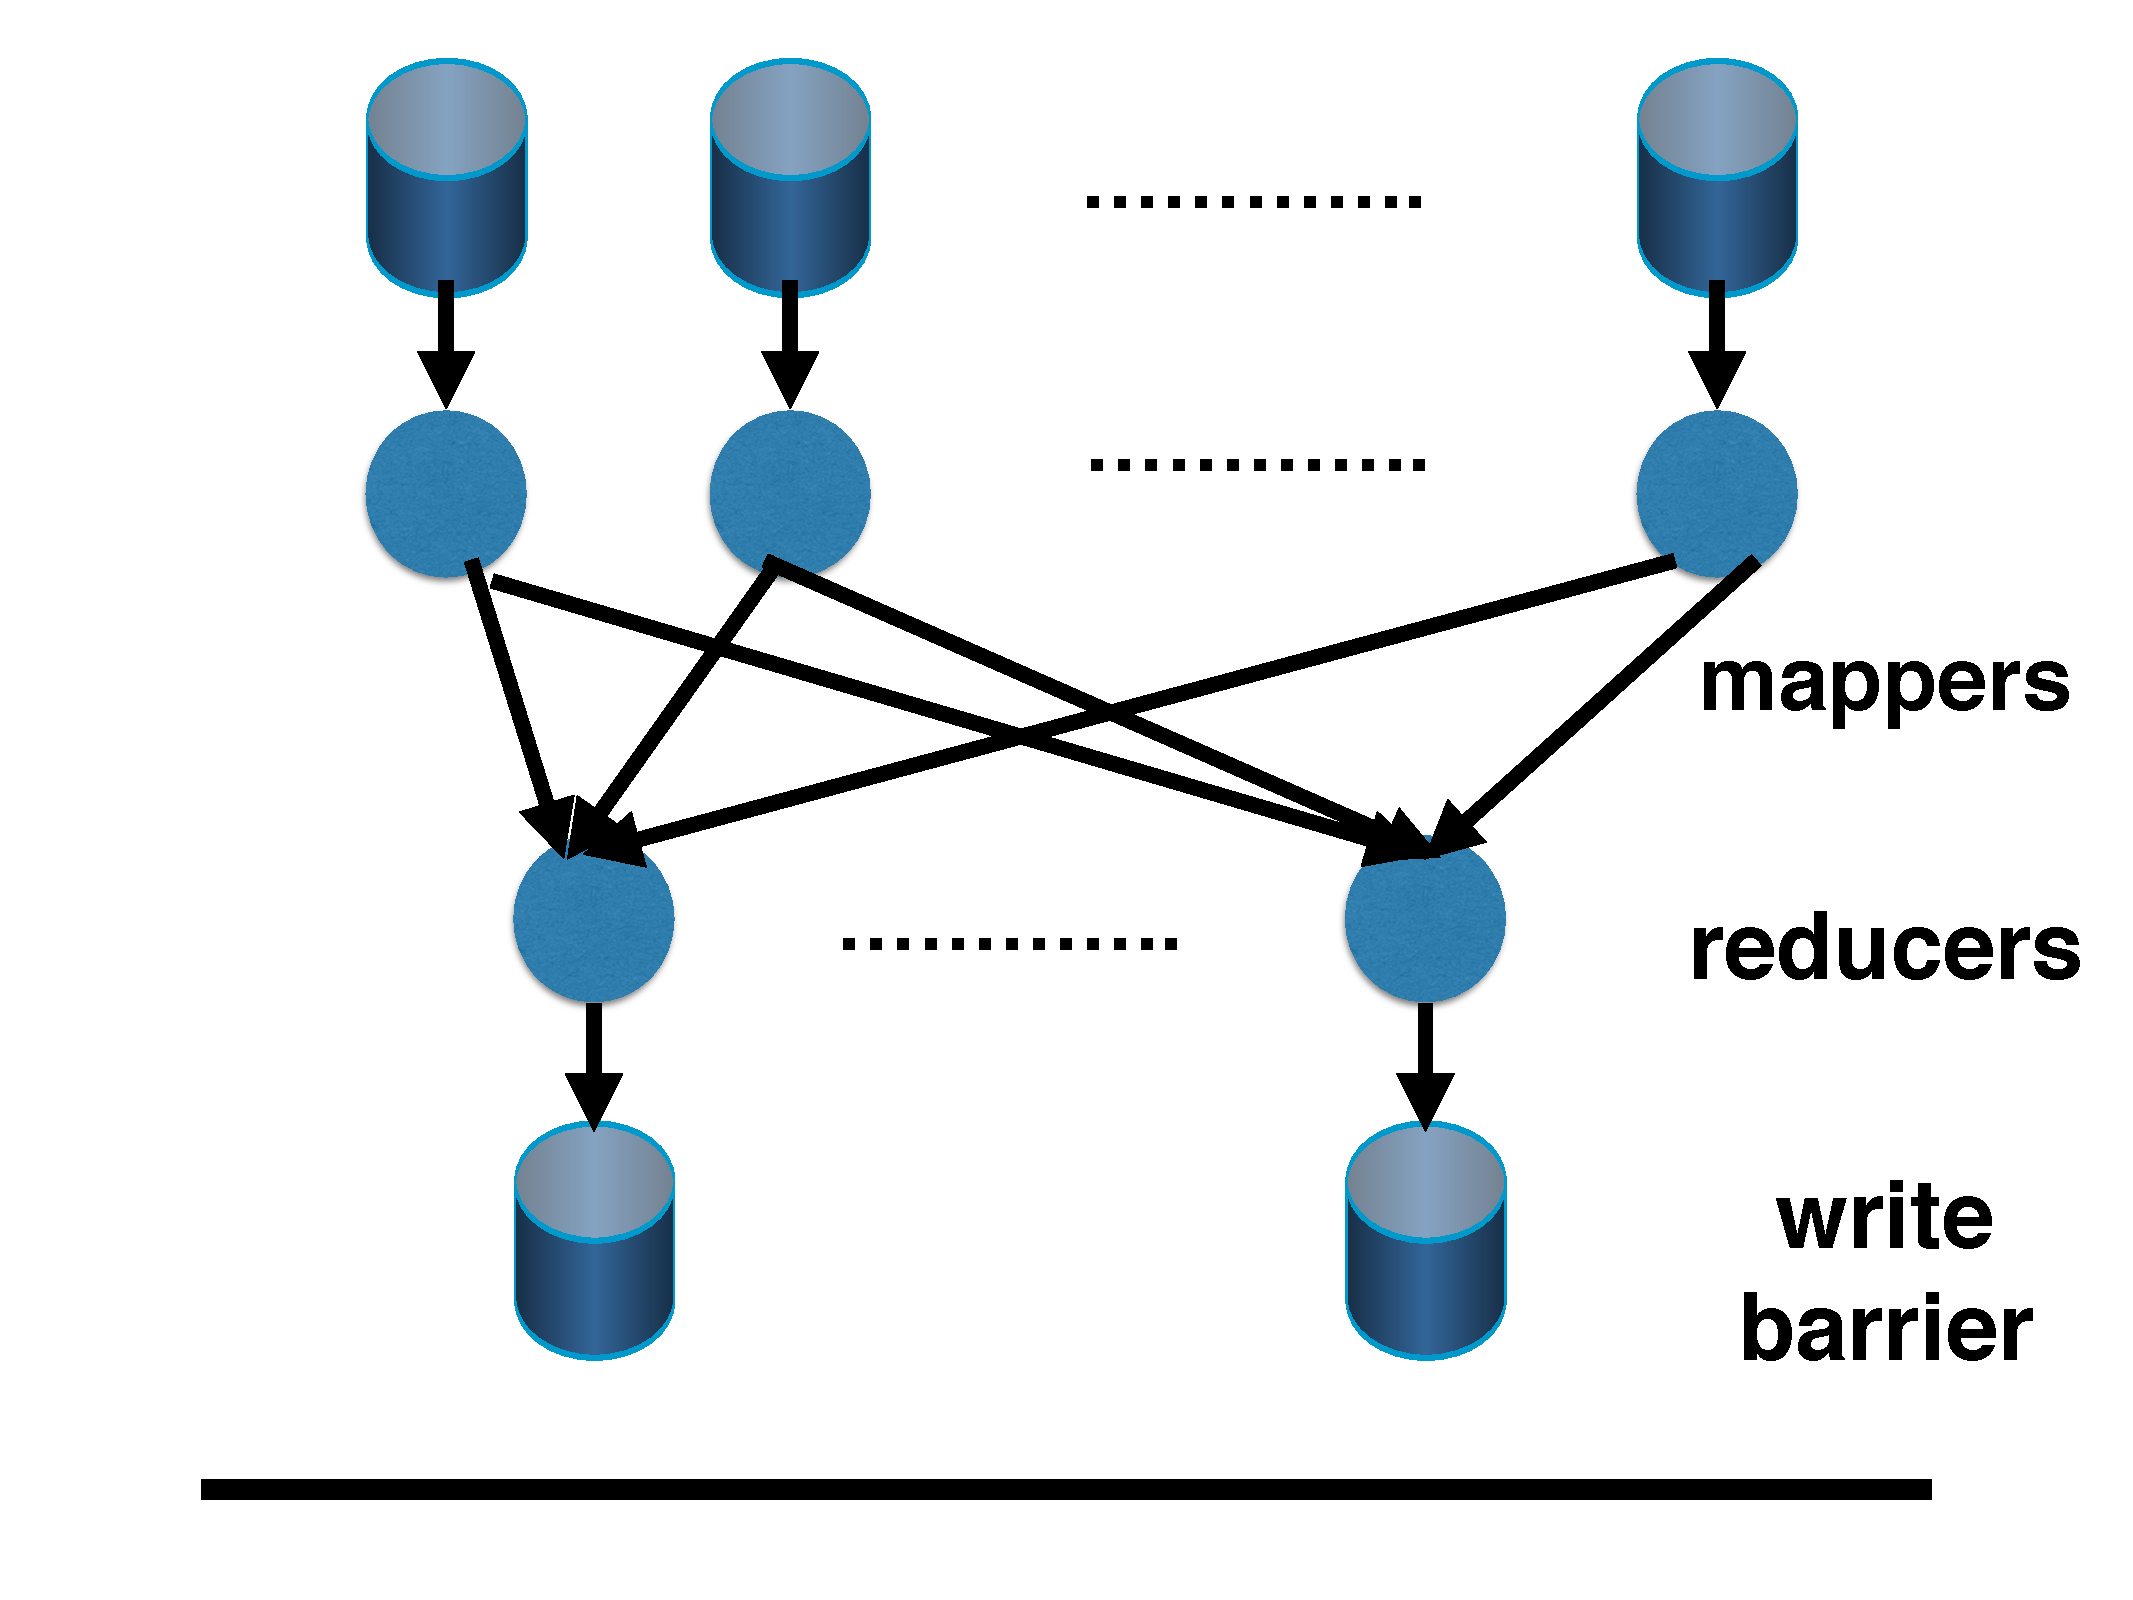
\includegraphics[width=0.48\columnwidth]{figures/others/map-reduce.pdf}}
  \subcaptionbox{带有阻碍的数据流}
      {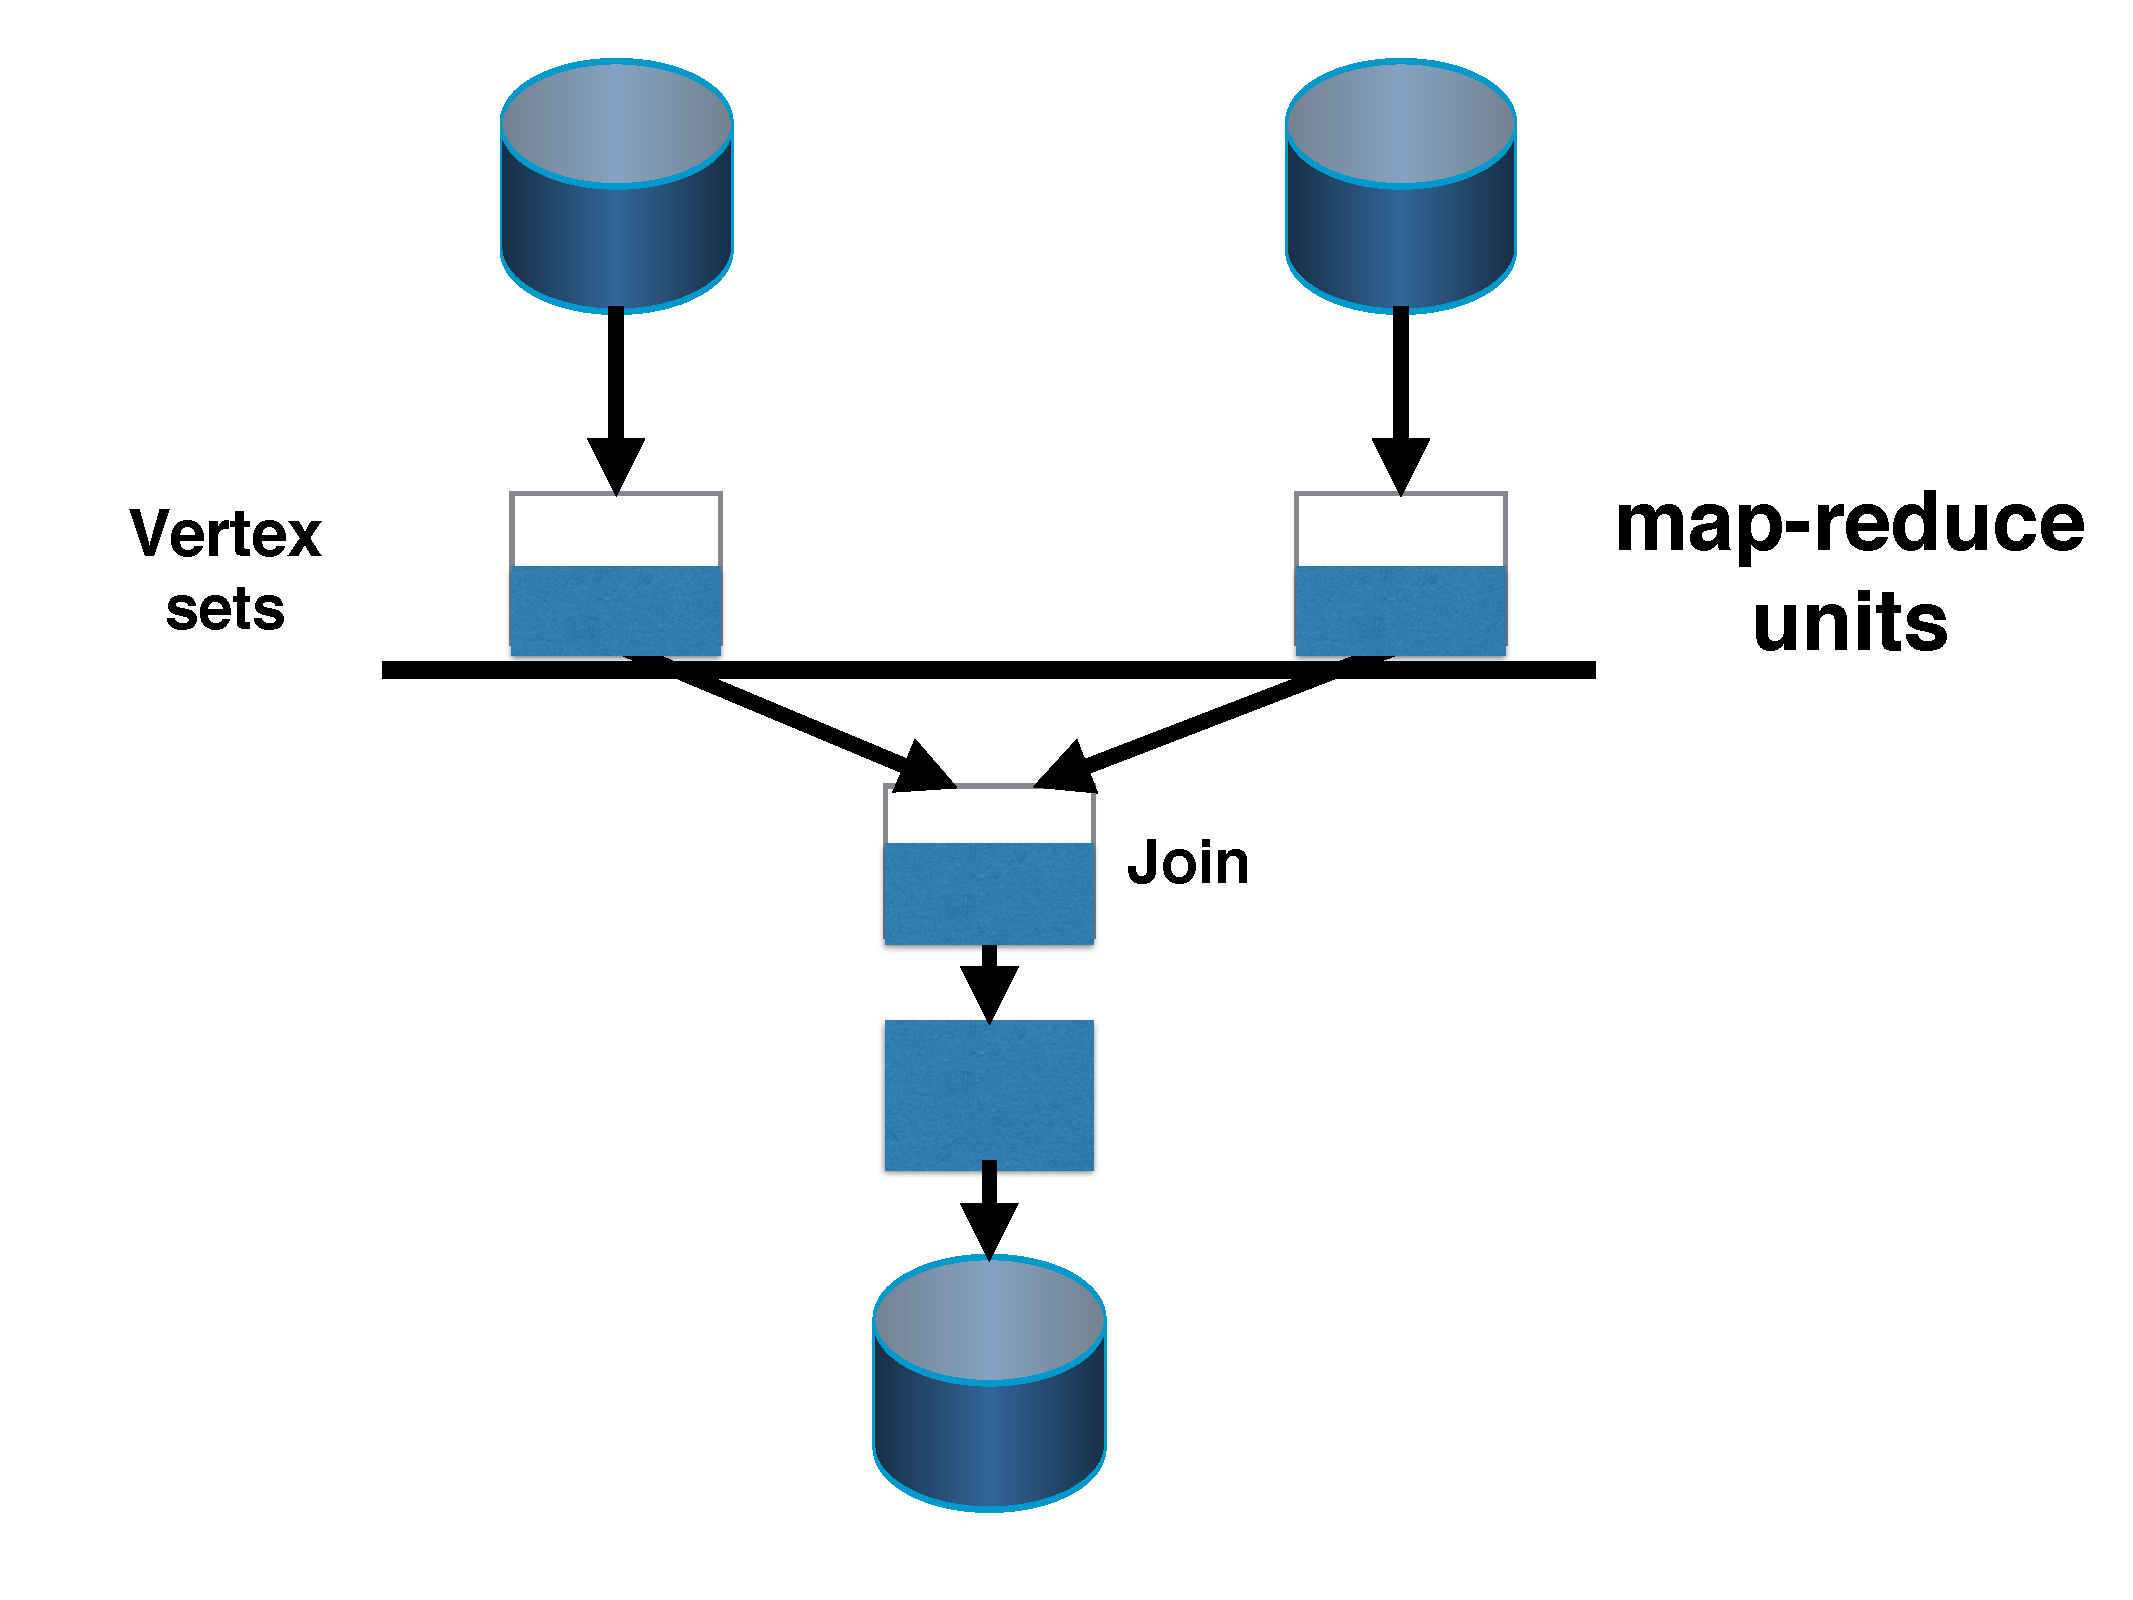
\includegraphics[width=0.48\columnwidth]{figures/others/vertex2.pdf}}
  \subcaptionbox{没有显示阻碍的数据流}
    {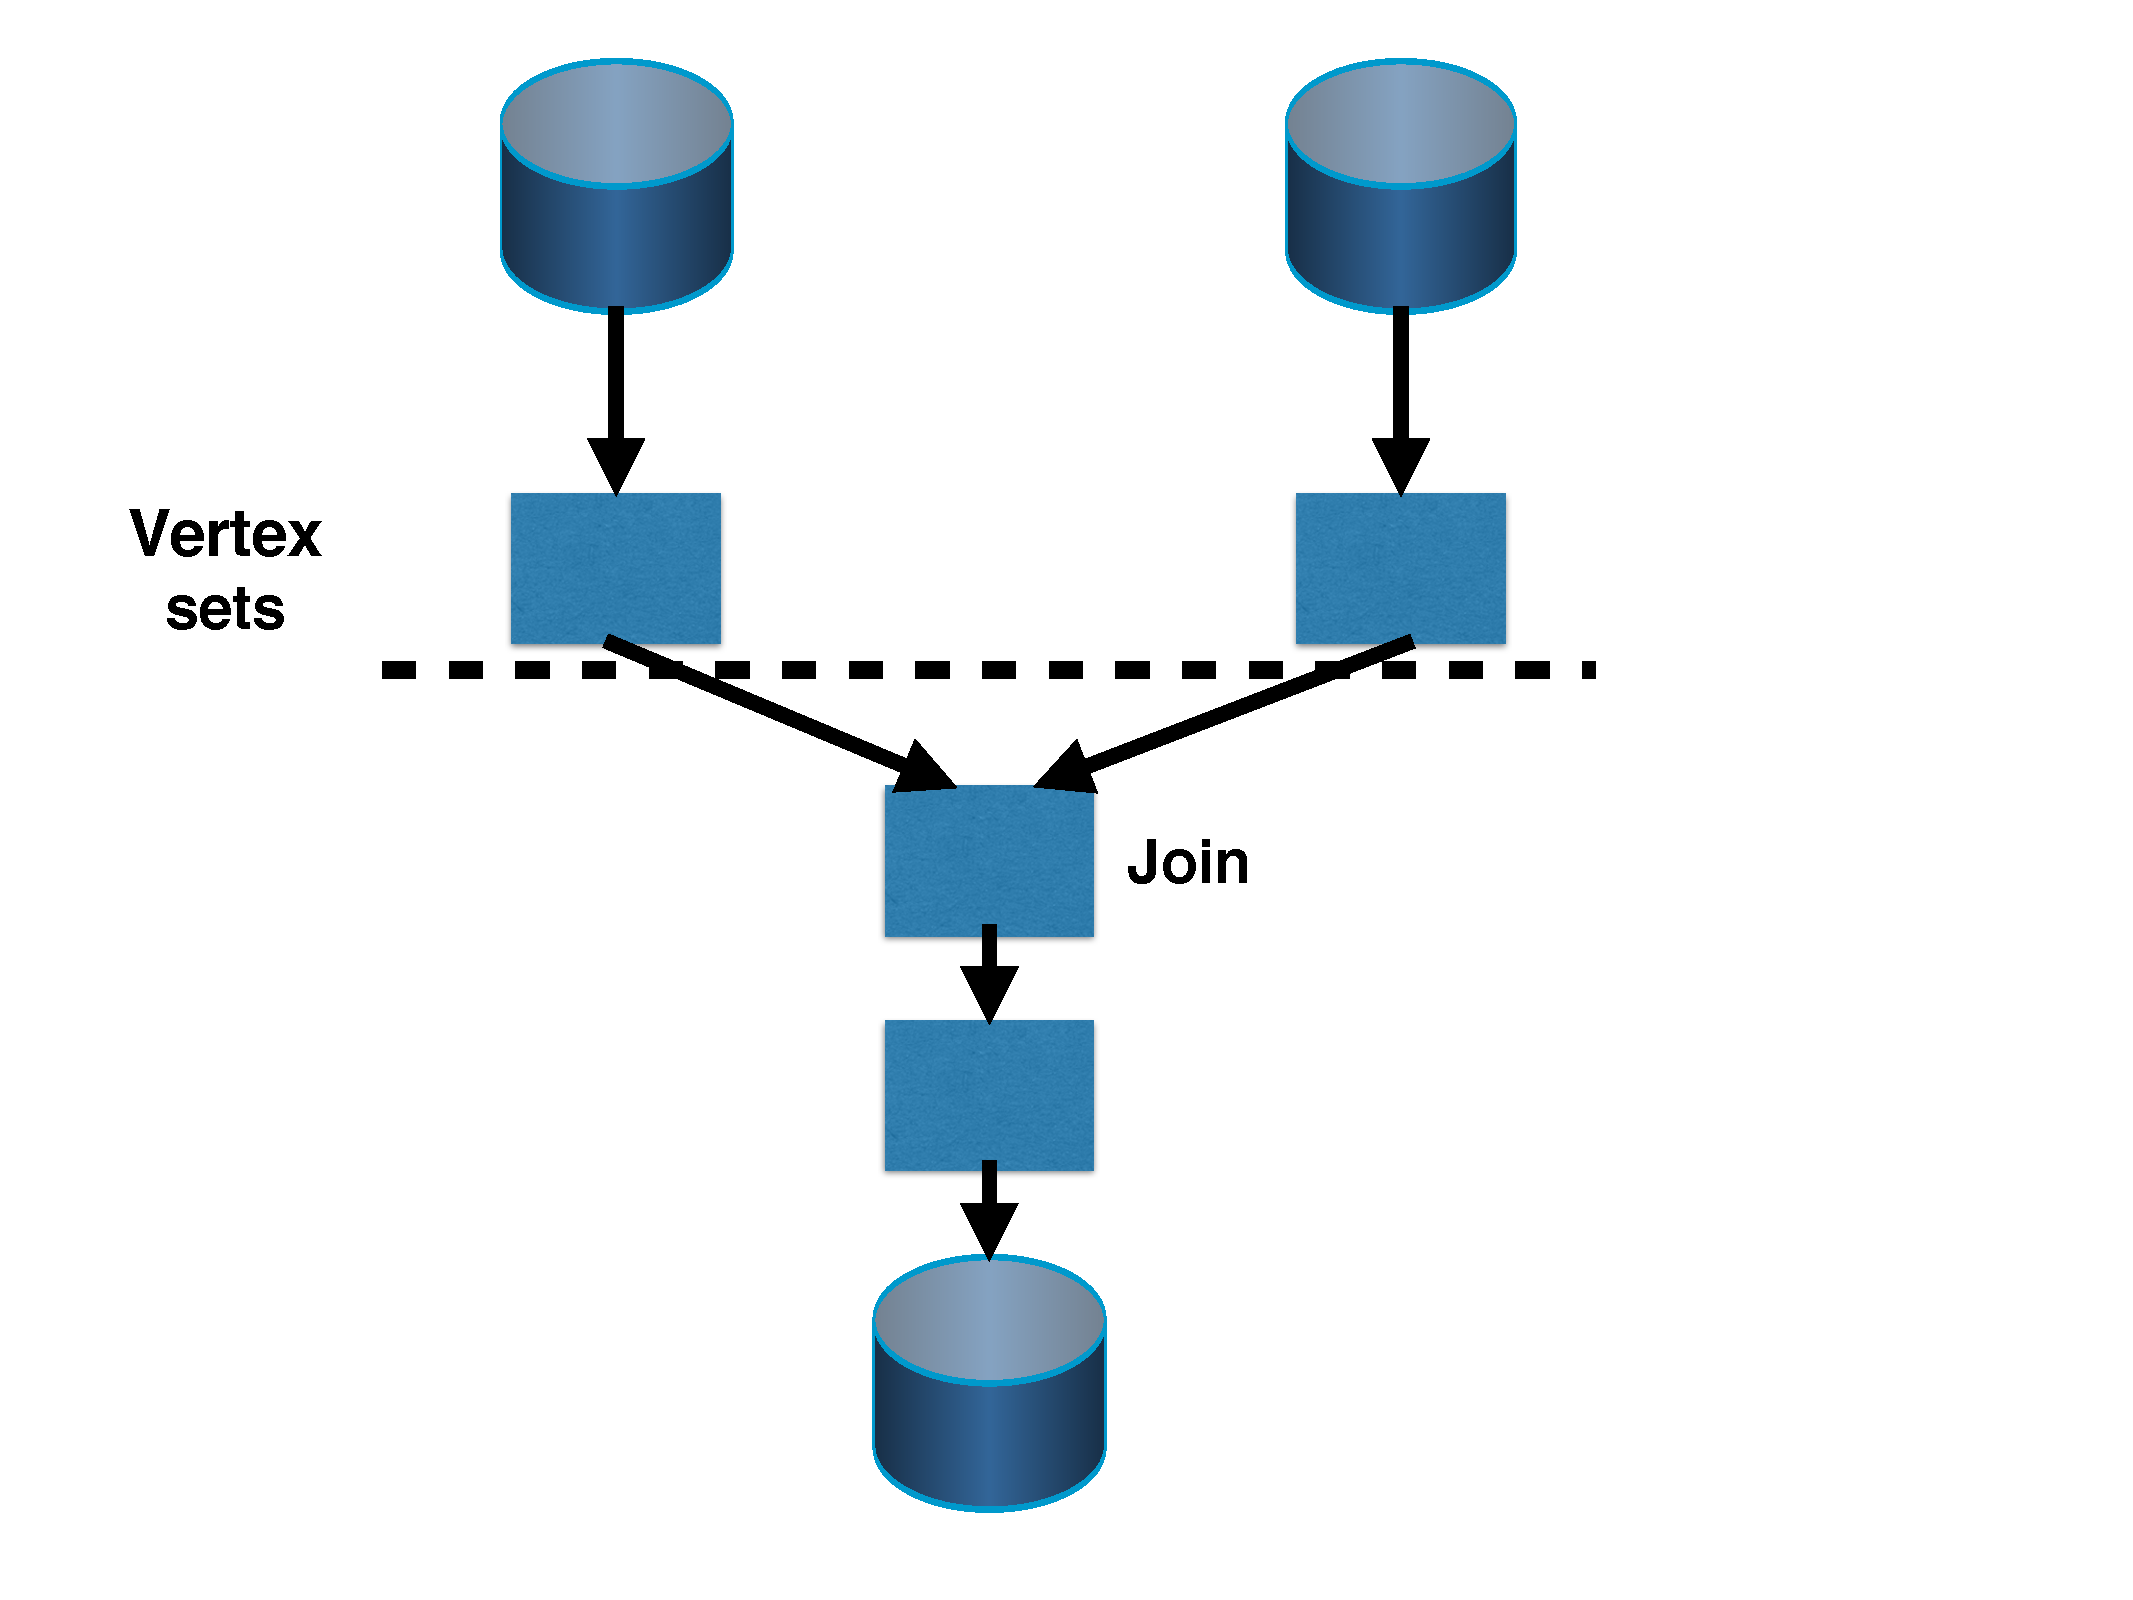
\includegraphics[width=0.48\columnwidth]{figures/others/vertex.pdf}}
  \subcaptionbox{环形数据流}
      {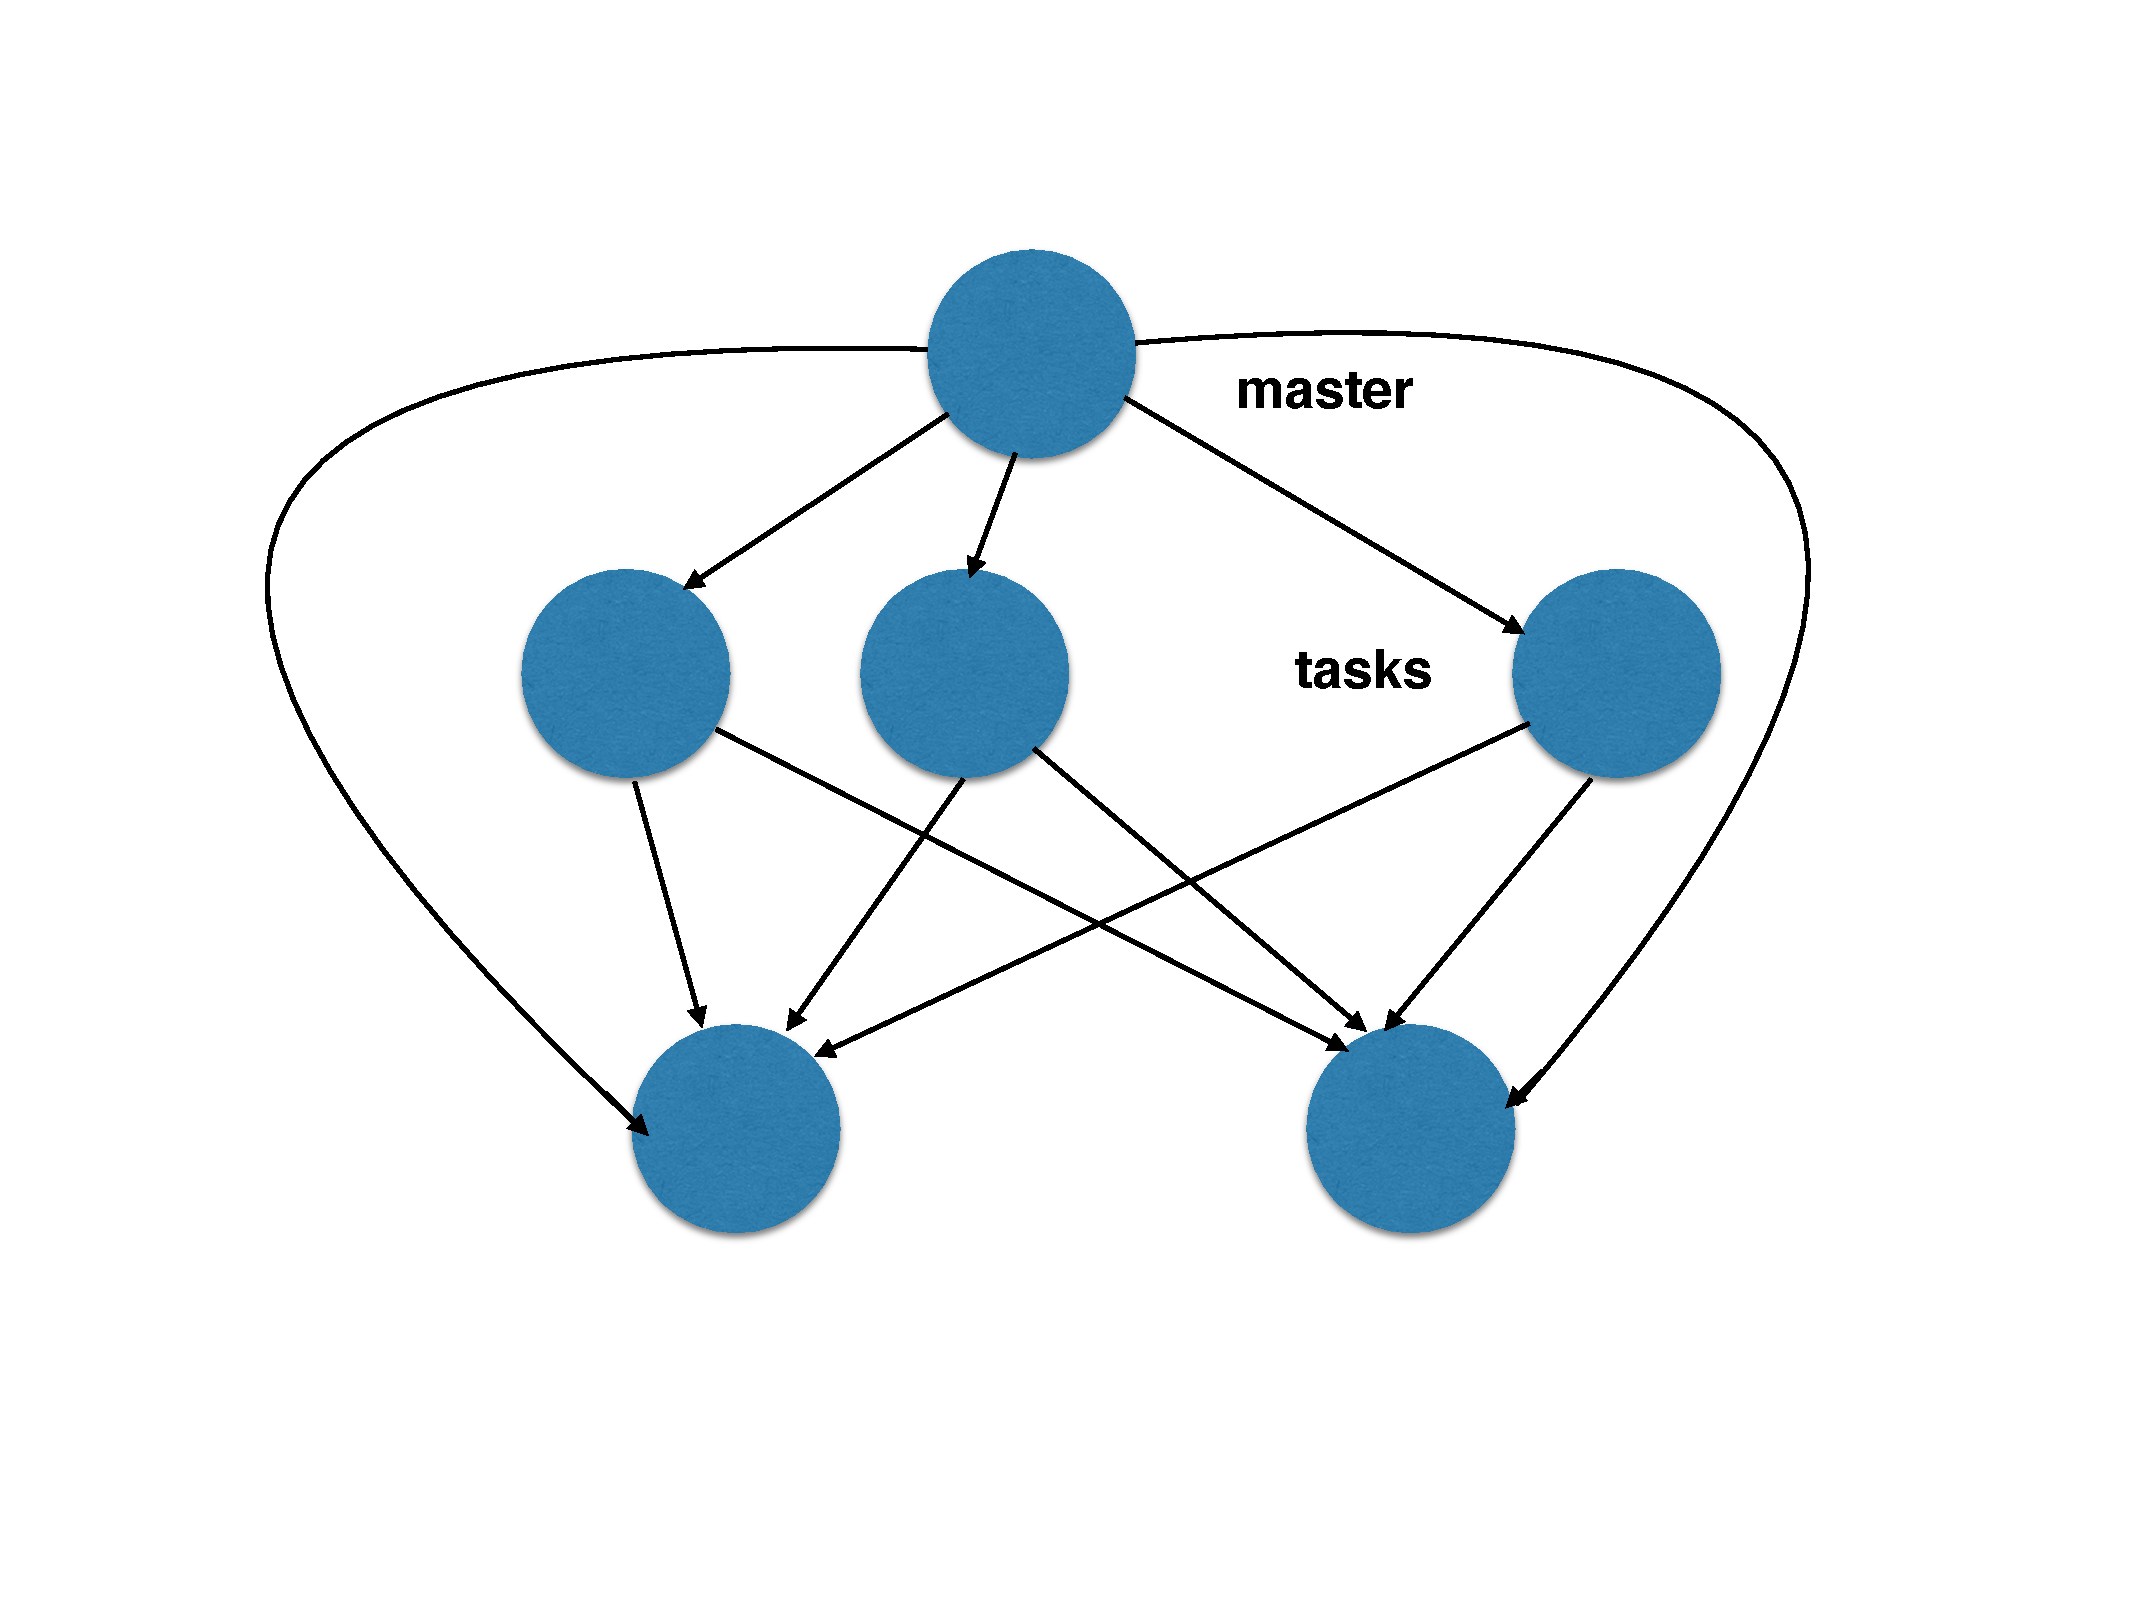
\includegraphics[width=0.48\columnwidth]{figures/others/Dataflow.pdf}}
   \subcaptionbox{并行大块数据流传输}
      {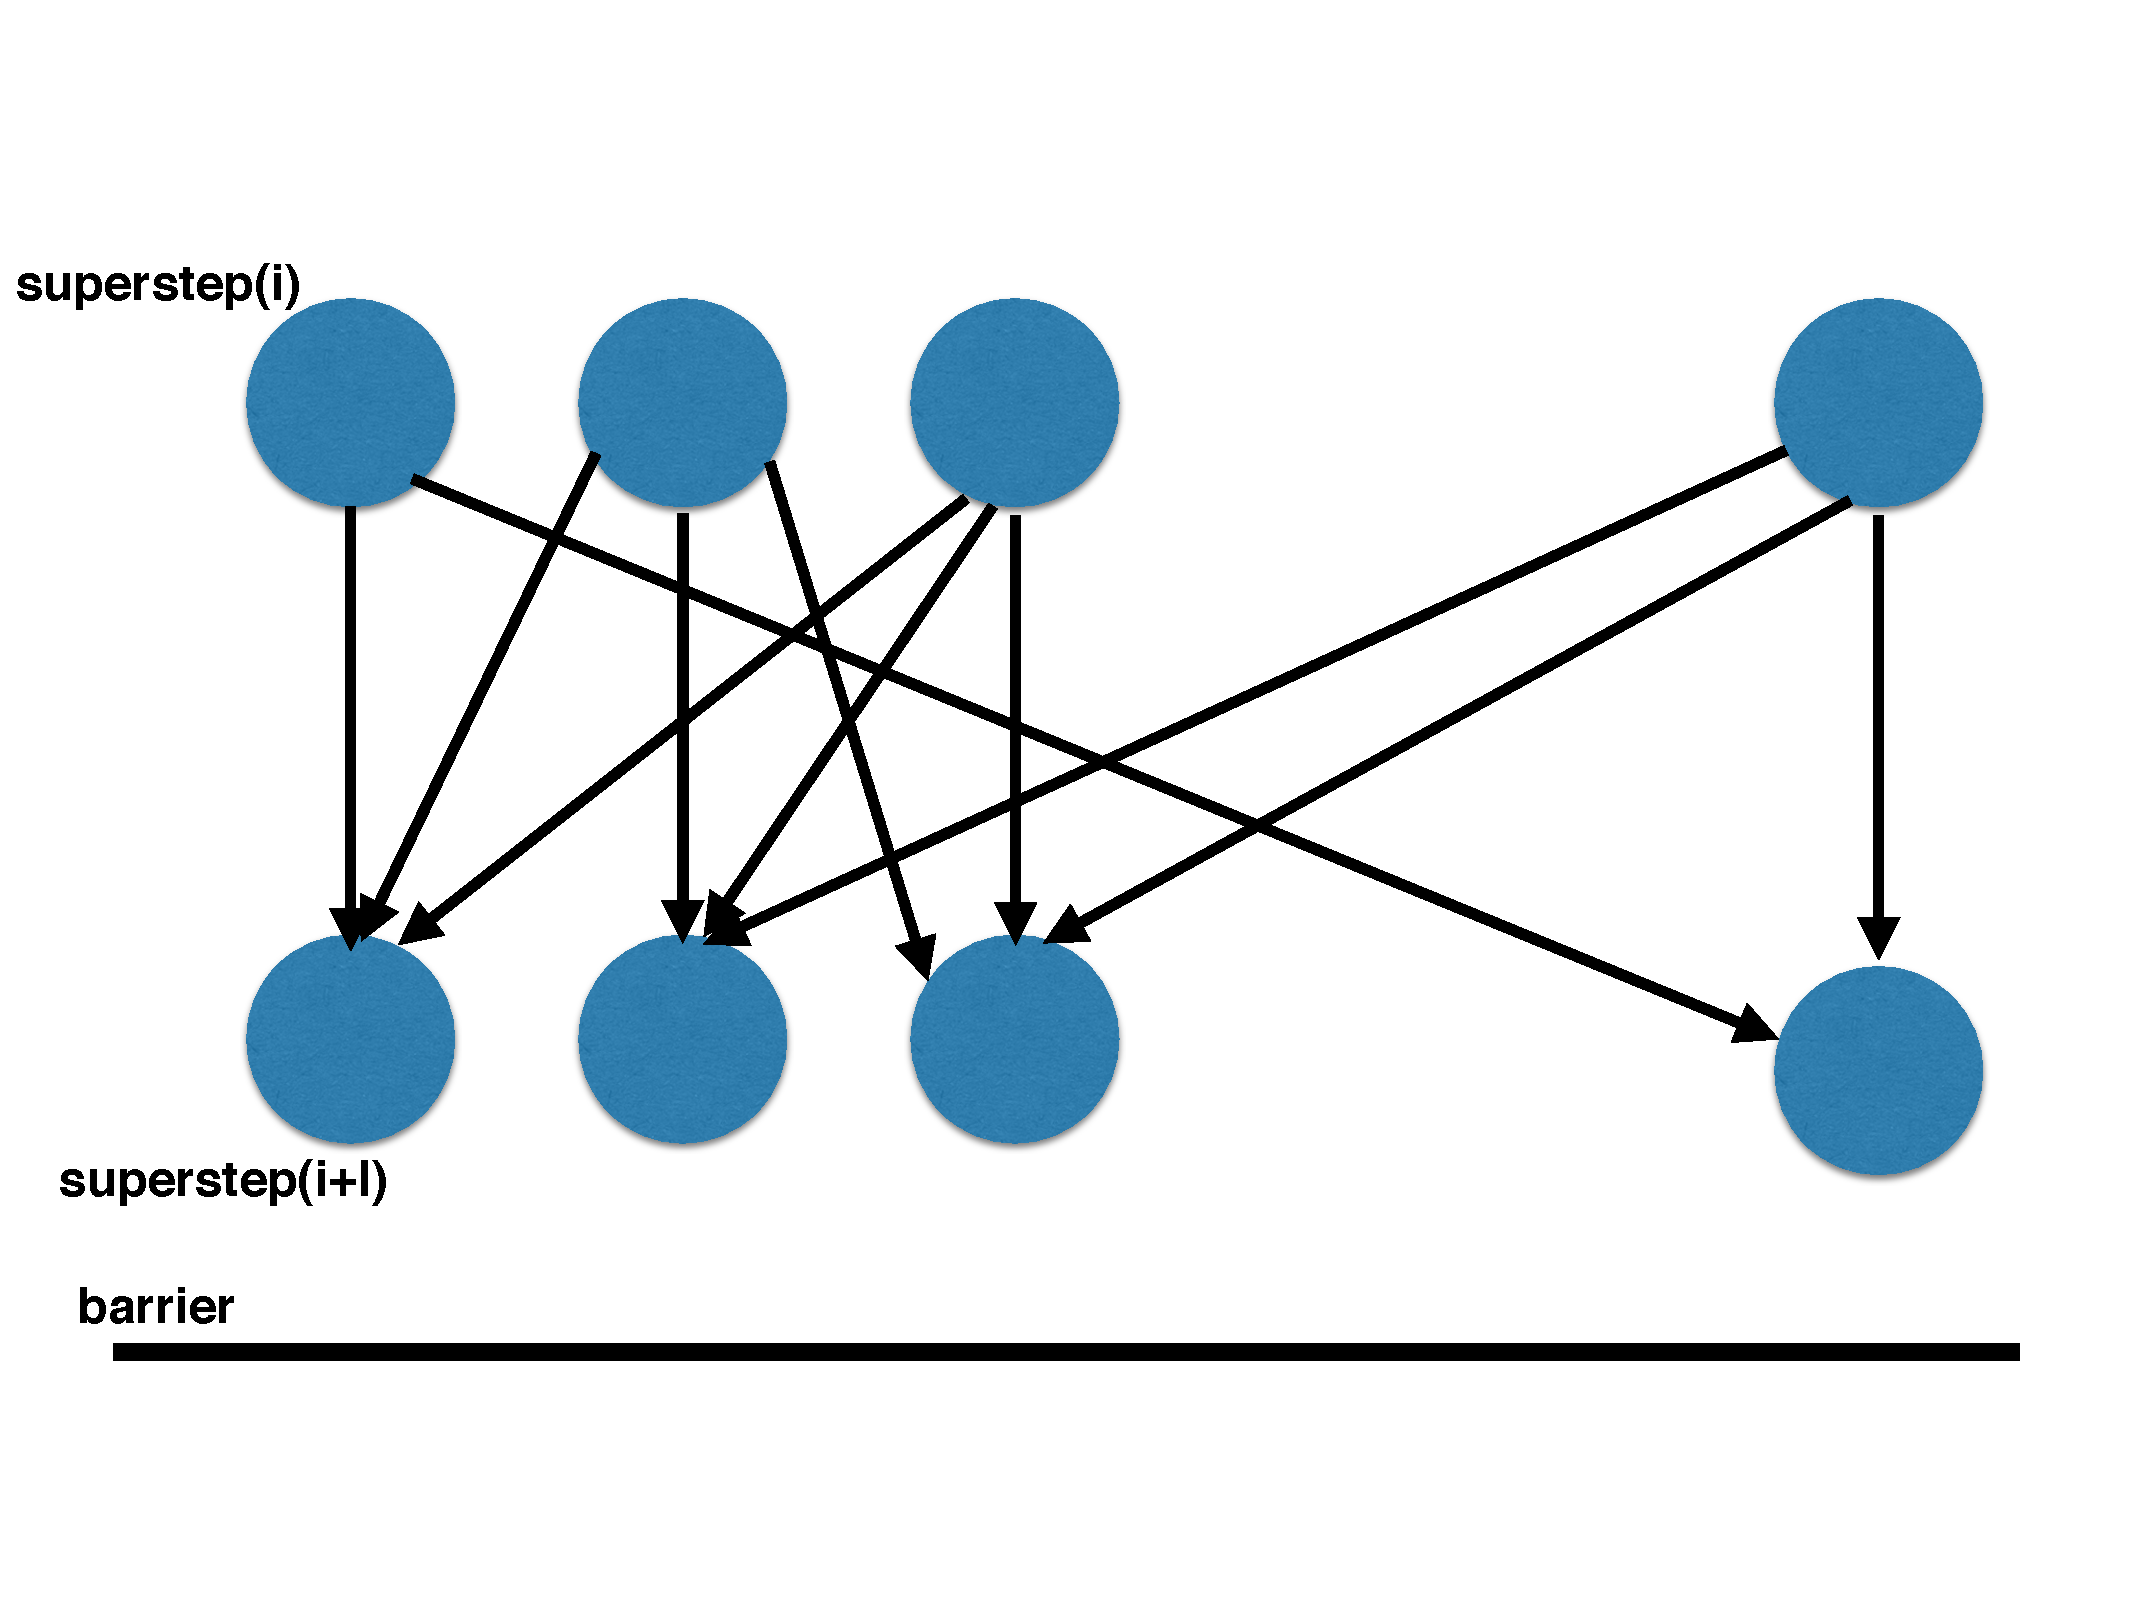
\includegraphics[width=0.48\columnwidth]{figures/others/BSP.pdf}}
   \subcaptionbox{分区-聚合}
      {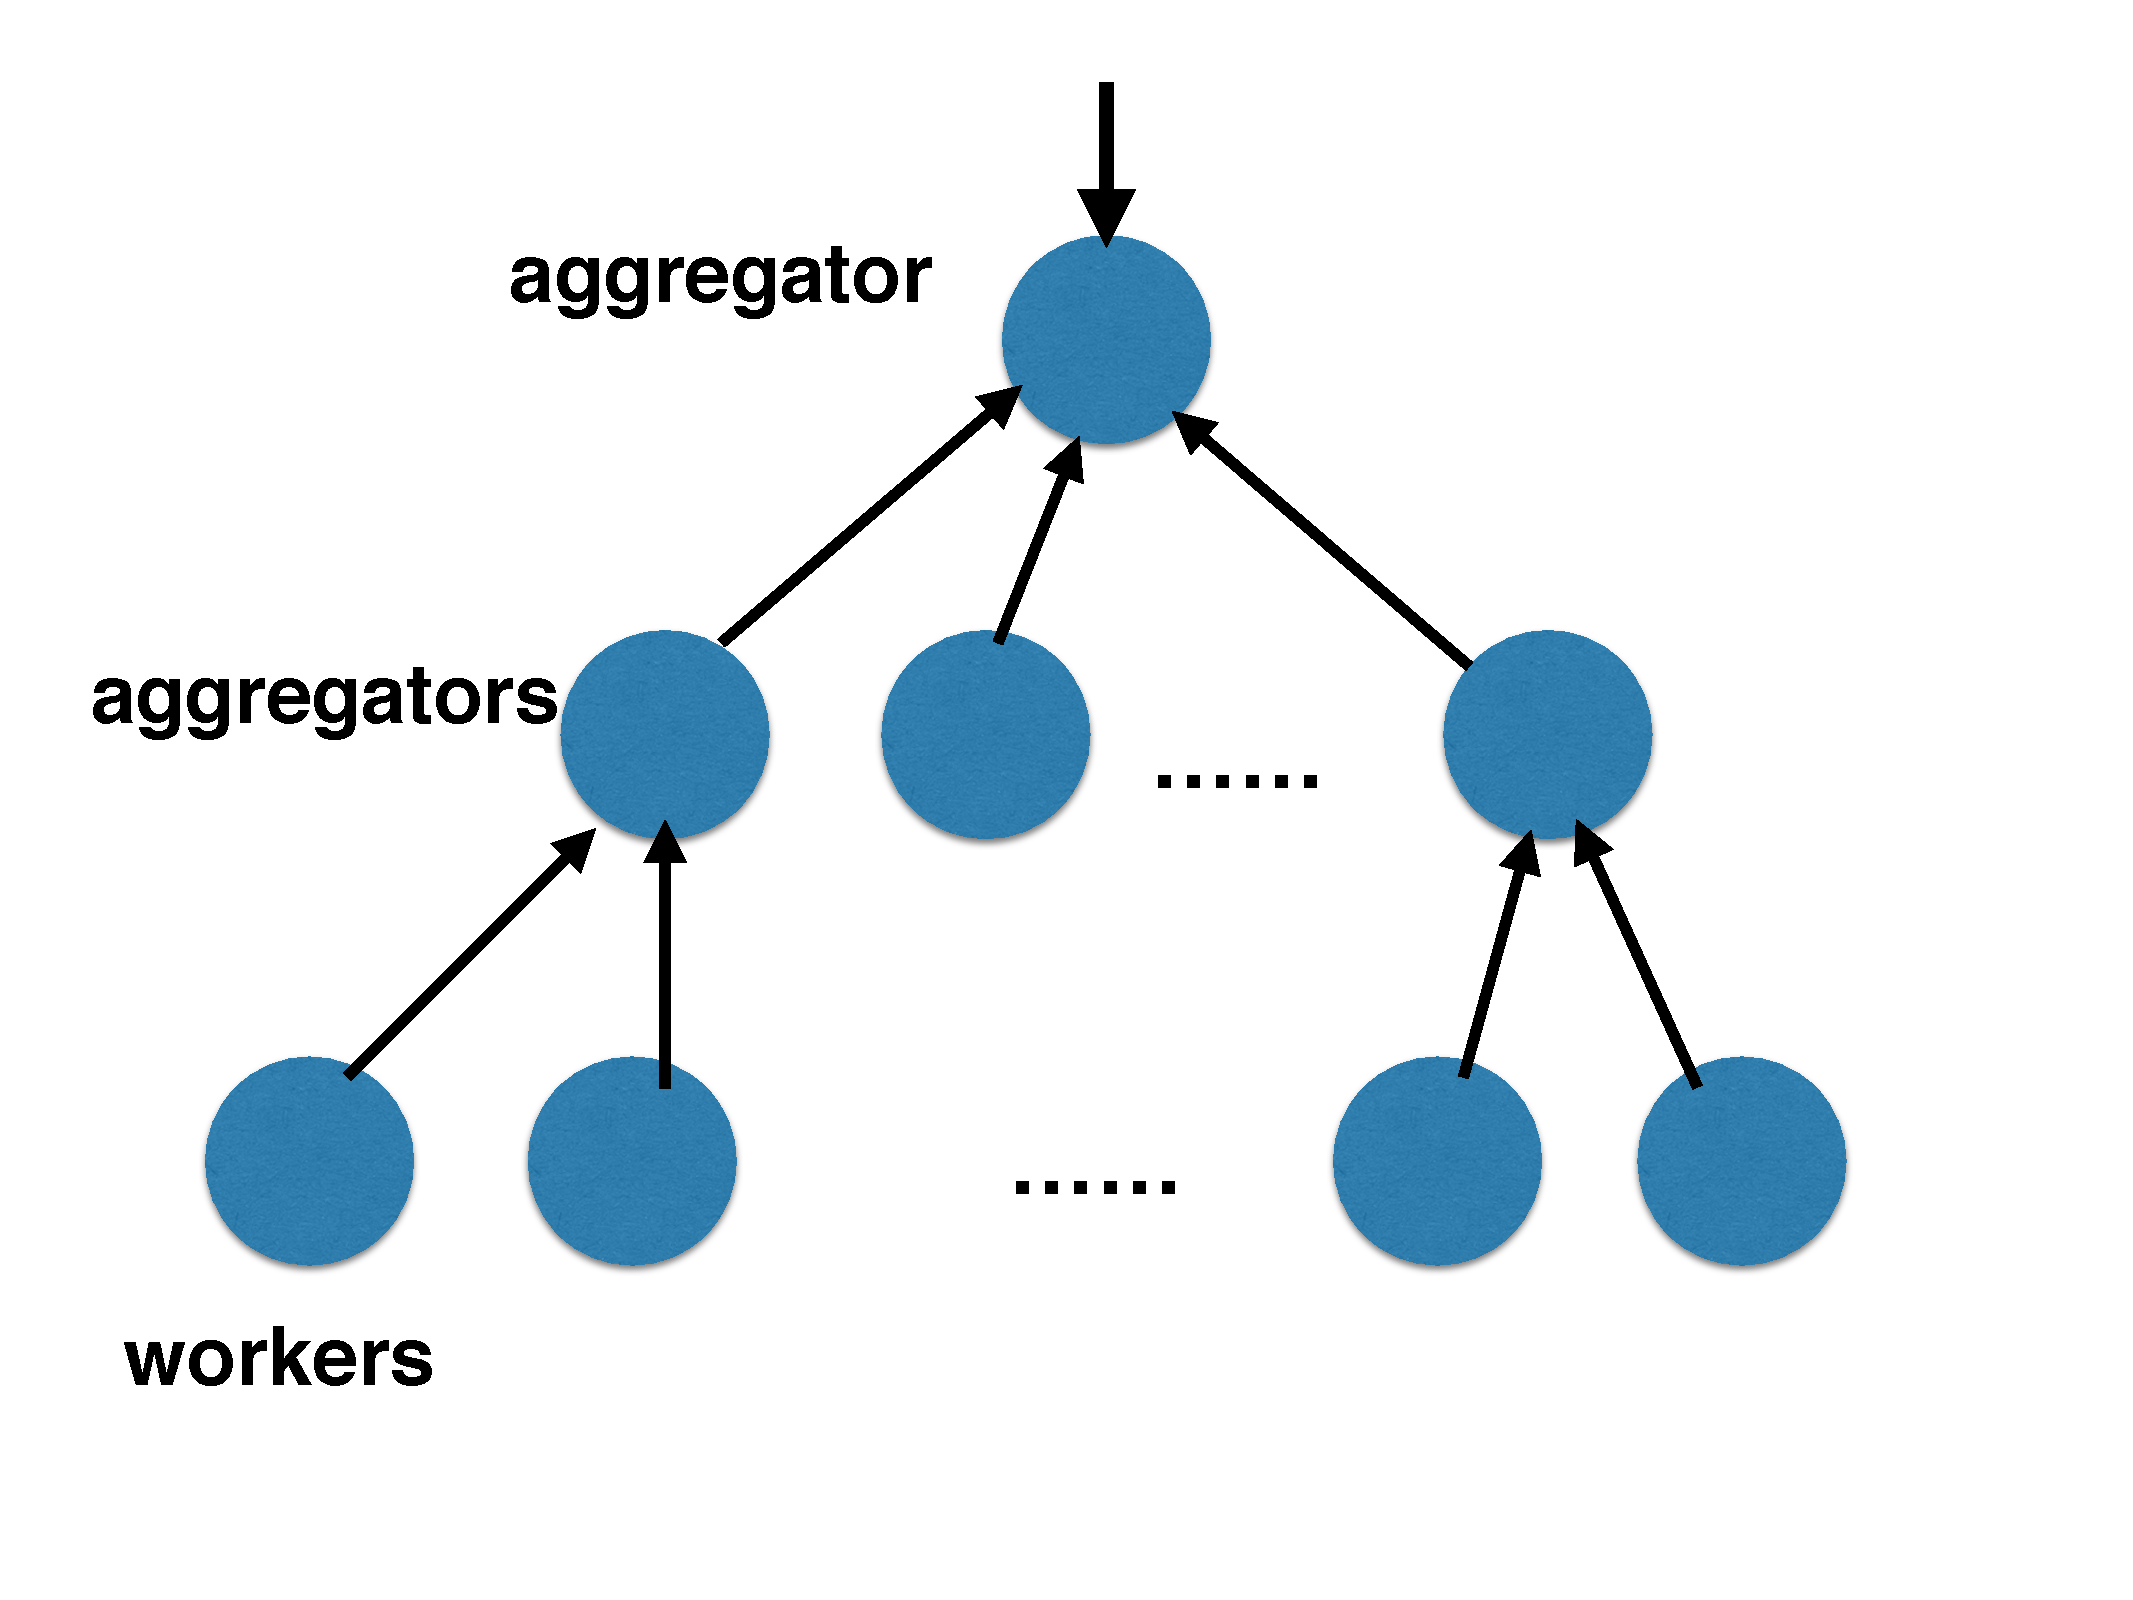
\includegraphics[width=0.48\columnwidth]{figures/others/partition-aggregate.pdf}}
  \caption{分布式应用的通信模型}
  \label{relatedwork-communication-fig}
\end{figure}


大多数集群应用程序的计算框架都是输入特定的配置参数,然后使用特定的计算模型,得到计算结果。
计算过程中,常常产生大量的数据,节点之间会进行频繁通信,不同的计算模型常有不同的通信模式,
这些通信模式可以总结成不同的通信模型。
图\ref{relatedwork-communication-fig}显示了6种通信模型,这些通信模型可以分成4类:
映射规约模型(Map-Reduce),数据流模型(Dataflow),
大型并行数据传输模型(Bulk Synchronous Parallel ),分区-聚合模型(Partition-Aggregate)。

\subsubsection{映射规约模型(Map-Reduce)}
MapReduce\cite{Dean2004Simplified}是一个众所周知的集群计算框架。
如图\ref{relatedwork-communication-fig}(a)所示,
每个mapper都从分布式文件系统(DFS)中读取输入,执行用户定义的计算,并将中间数据写到磁盘上;
每个reducer都从不同的mapper中提取中间数据,将它们合并,并将其输出写入DFS。

给定m个mappers和r个reducer,MapReduce的shuffle阶段将产生总数为$m\times r$条数据流。
经过reducer处理完毕以后,至少有r条数据流被复制。
MapReduce模型中shuffle阶段会产生很多并行的数据流,
直到最后一条数据流传输结束此传输过程才会传输完毕。
因此,在任务传输的最后阶段,有一个显式的同步。
有研究\cite{Chowdhury2011Managing}针对MapReduce存在任务数据流同步的特点,
优化了shuffle阶段的传输,以此来提高传输的性能。

\subsubsection{数据流模型(Dataflow)}
虽然MapReduce被广泛使用,但是因为其存在数据阻塞等问题,常常会影响应用的整体性能。
Dataflow通信模型的出现解决了MapReduce很多的不足,
数据流模型有以下三种方式:

\textbf{带有阻塞的数据流模型}。
如图\ref{relatedwork-communication-fig}(b)所示,
有的多阶段的数据流模型使用MapReduce作为其构建模块(例如,Hive\footnote{Apache Hive.~http://hadoop.apache.org/hive/.},Pig\cite{Olston2008Pig})。
因为基于MapReduce,因此,MapReduce类似,带有阻塞的Dataflow的通信模型在每个构建模块的末尾都有同步操作。

\textbf{无阻塞的数据流模型}。
如图\ref{relatedwork-communication-fig}(c)所示,
一些数据流模型并没有明显的同步操作(比如Dryad\cite{Isard2007Dryad},DryadLINQ\cite{Yu2008DryadLINQ},SCOPE\cite{Chaiken2008SCOPE},FlumeJava\cite{Chambers2010FlumeJava})。
当输入的数据准备好以后,下一个阶段就会开始。
因为没有明确的同步操作,
所以针对MapReduce等存在同步框架的优化技术对此通信框架没有任何效果。
因此,很多研究人员针对采用没有显式阻塞的数据流通信模式的应用进行了特殊优化处理\cite{Guo2015Spotting,Zhang2012Optimizing}。

\textbf{环形数据流模型}。
如图\ref{relatedwork-communication-fig}(d)所示的是环形数据流通信模型。
和无阻塞的数据流模型不同的是,在环形数据流中,数据流会重复使用之前阶段的部分组件。
因为不同的阶段的数据流传输会复用组件,因此,可能会引起组件使用的冲突。
Spark\cite{Zaharia2012Resilient}通过在迭代中保留内存状态来消除循环冲突带来的开销。

\subsubsection{大型并行数据传输模型(Bulk Synchronous Parallel )}
大型并行数据传输模型(Bulk Synchronous Parallel,简称BSP )是集群计算中的另一个众所周知的通信模型。
使用这种模型的框架包括Pregel\cite{Malewicz2010Pregel}、
Giraph\footnote{Apache Giraph.~http://incubator.apache.org/giraph/.}和Hama\footnote{Apache Hama.~http://hama.apache.org.}等,
许多图形处理、矩阵计算等工具使用BSP框架。
如图\ref{relatedwork-communication-fig}(e)所示,
BSP计算在一系列全局superstep中进行,
每个superstep包含三个有序阶段:并行计算、进程通信和同步数据。
在每一个superstep的末尾有明确的同步操作。

\subsubsection{分区-聚合模型(Partition-Aggregate)}
图\ref{relatedwork-communication-fig}(f)显示是数据中心分区-聚合模型(Partition-Aggregate)。
分区-聚合模型是很多大型分布式计算通信模型。
在分区-聚合模型中,请求发送到根节点,根节点把请求下发给底部的worker节点。
随后,worker节点把结果聚集到一起,然后把计算完成的结果,反馈给根节点。
在数据中心,网络搜索、社交网络内容组成和广告选择等应用的通信模式均是基于此模式设计的。
对于交互式的、实时的应用,用户得到响应的延迟是衡量服务质量好坏的重要指标。
在减去传输等延迟之后,留给计算的时间通常只有230$\sim$300毫秒。

许多应用采用多层的分区-聚合模式,其中一个层的传输延迟会影响另一个层的启动。
此外,响应请求可能需要迭代地调用,一个aggregator节点向下面的worker节点发出连续的请求,
以准备响应(1到4次响应是常见的,甚至有时能到20次)。
例如,在web搜索中,一个查询会发送给许多aggregator和worker,每个组件负责不同的部分。
根据回复,聚合器可能会细化查询并再次发送,以增加结果的完备性。
因此,分区-聚合传输延迟过高会增加对查询结果性能的影响。


为了防止SLA(Service Level Agreement)性能被破坏,
常常需要给worker节点设置一个截止期限(deadline),截止期限通常在10ms$\sim$100ms。
当一个worker节点错过了截止期限时,上层aggregator节点将会收到不完整的结果,这样会使的计算结果受到影响。
因此,对于用户来说,越来越多的的流在截止期限之前完成对用户体验十分重要。
例如,可能有$99.9\%$的流在截止期限之前完成,意味着,1000个请求中,有1个请求不能在截止时间之前完成。
这样会严重影响用户的体验,造成客户的流失,造成不可逆转的损失。

\subsection{网络流量特征分析}

随着数据中心中部署应用的增多,对数据中心中流量特性的研究也逐渐增多。
本部分对当前业界对数据中心流量测量的工作进行了总结和归纳。




\textbf{查询流}。查询流常常是由类似web这类请求产生的,这种请求的通信模型常常是Partition-Aggregage。
查询流非常短,并且对延迟十分敏感。
当一个用户请求到达上层aggregator的节点时,上层的网络节点把请求下发给中层的节点,计算结果后,然后再下发给下层的worker节点。
worker节点得到请求后,读取请求的内容,然后计算结果,
随后把结果反馈给根节点,根节点根据得到的反馈结果,进行处理。
查询流的规模是非常有规律的,从高层的根节点到下层的worker节点的查询流的大小约为1.6KB,
从子节点回馈给根节点的流大小大约是1.6KB到2KB。





\textbf{背景流}。背景流和查询流共同存在于数据中心。
大多数背景流通常短于1MB,但是数据中心超过$90\%$的数据量来自约$1\%$的背景流。
这些长流通常在1MB到50MB之间。
在分布式模型中,有很多拷贝和更新节点状态的背景数据流,这些流大小在50KB到1MB。
背景流的到达间隔时间反映了应用的不同服务的叠加和应用的多样性。
背景流有如下的特性:
(1)流到达时间间隔跨度很大,流的到达是服从重尾分布,在较短的时间间隔内,会有大量背景数据流到达。
(2)长流发送是有一定周期性的,出现周期性是因为下层的叶节点会周期性的更新文件,此过程中会产生大量流。





\textbf{数据流并行程度和大小}。
在数据中心内,并行流数目的中位数为36。
$99\%$的机器之间连接数目在1600以内,有的机器连接的中位数,甚至在1200\cite{DCTCP}。
当只考虑长流($>$1MB时),机器之间并发的长流数目较少,并行的长流的平均数为1,
并且大约$75\%$的机器长流的并发数目在2以内。
这些流,能持续几个RTT,交换机的缓冲区大部分空间都是由这些流的数据包占据。

总之,对延迟敏感的查询流和需要高带宽的背景流同时存在于数据中心,
在数据中心,这些数据流对网络资源的需求不同,
我们需要设计合理的网络协议,来满足不同的流对网络资源的需求。

\textbf{关于期限}。Web应用的交互性意味着延迟是决定服务质量的关键。
研究表明,用户需要快速的回复响应\cite{kohavi2009controlled}。
除去节点之间网络传输时间,
应用通常具有200$\sim$300ms时间以完成其操作并对用户进行回复\cite{Decandia2007Dynamo}。

\begin{figure}[b]
\begin{center}
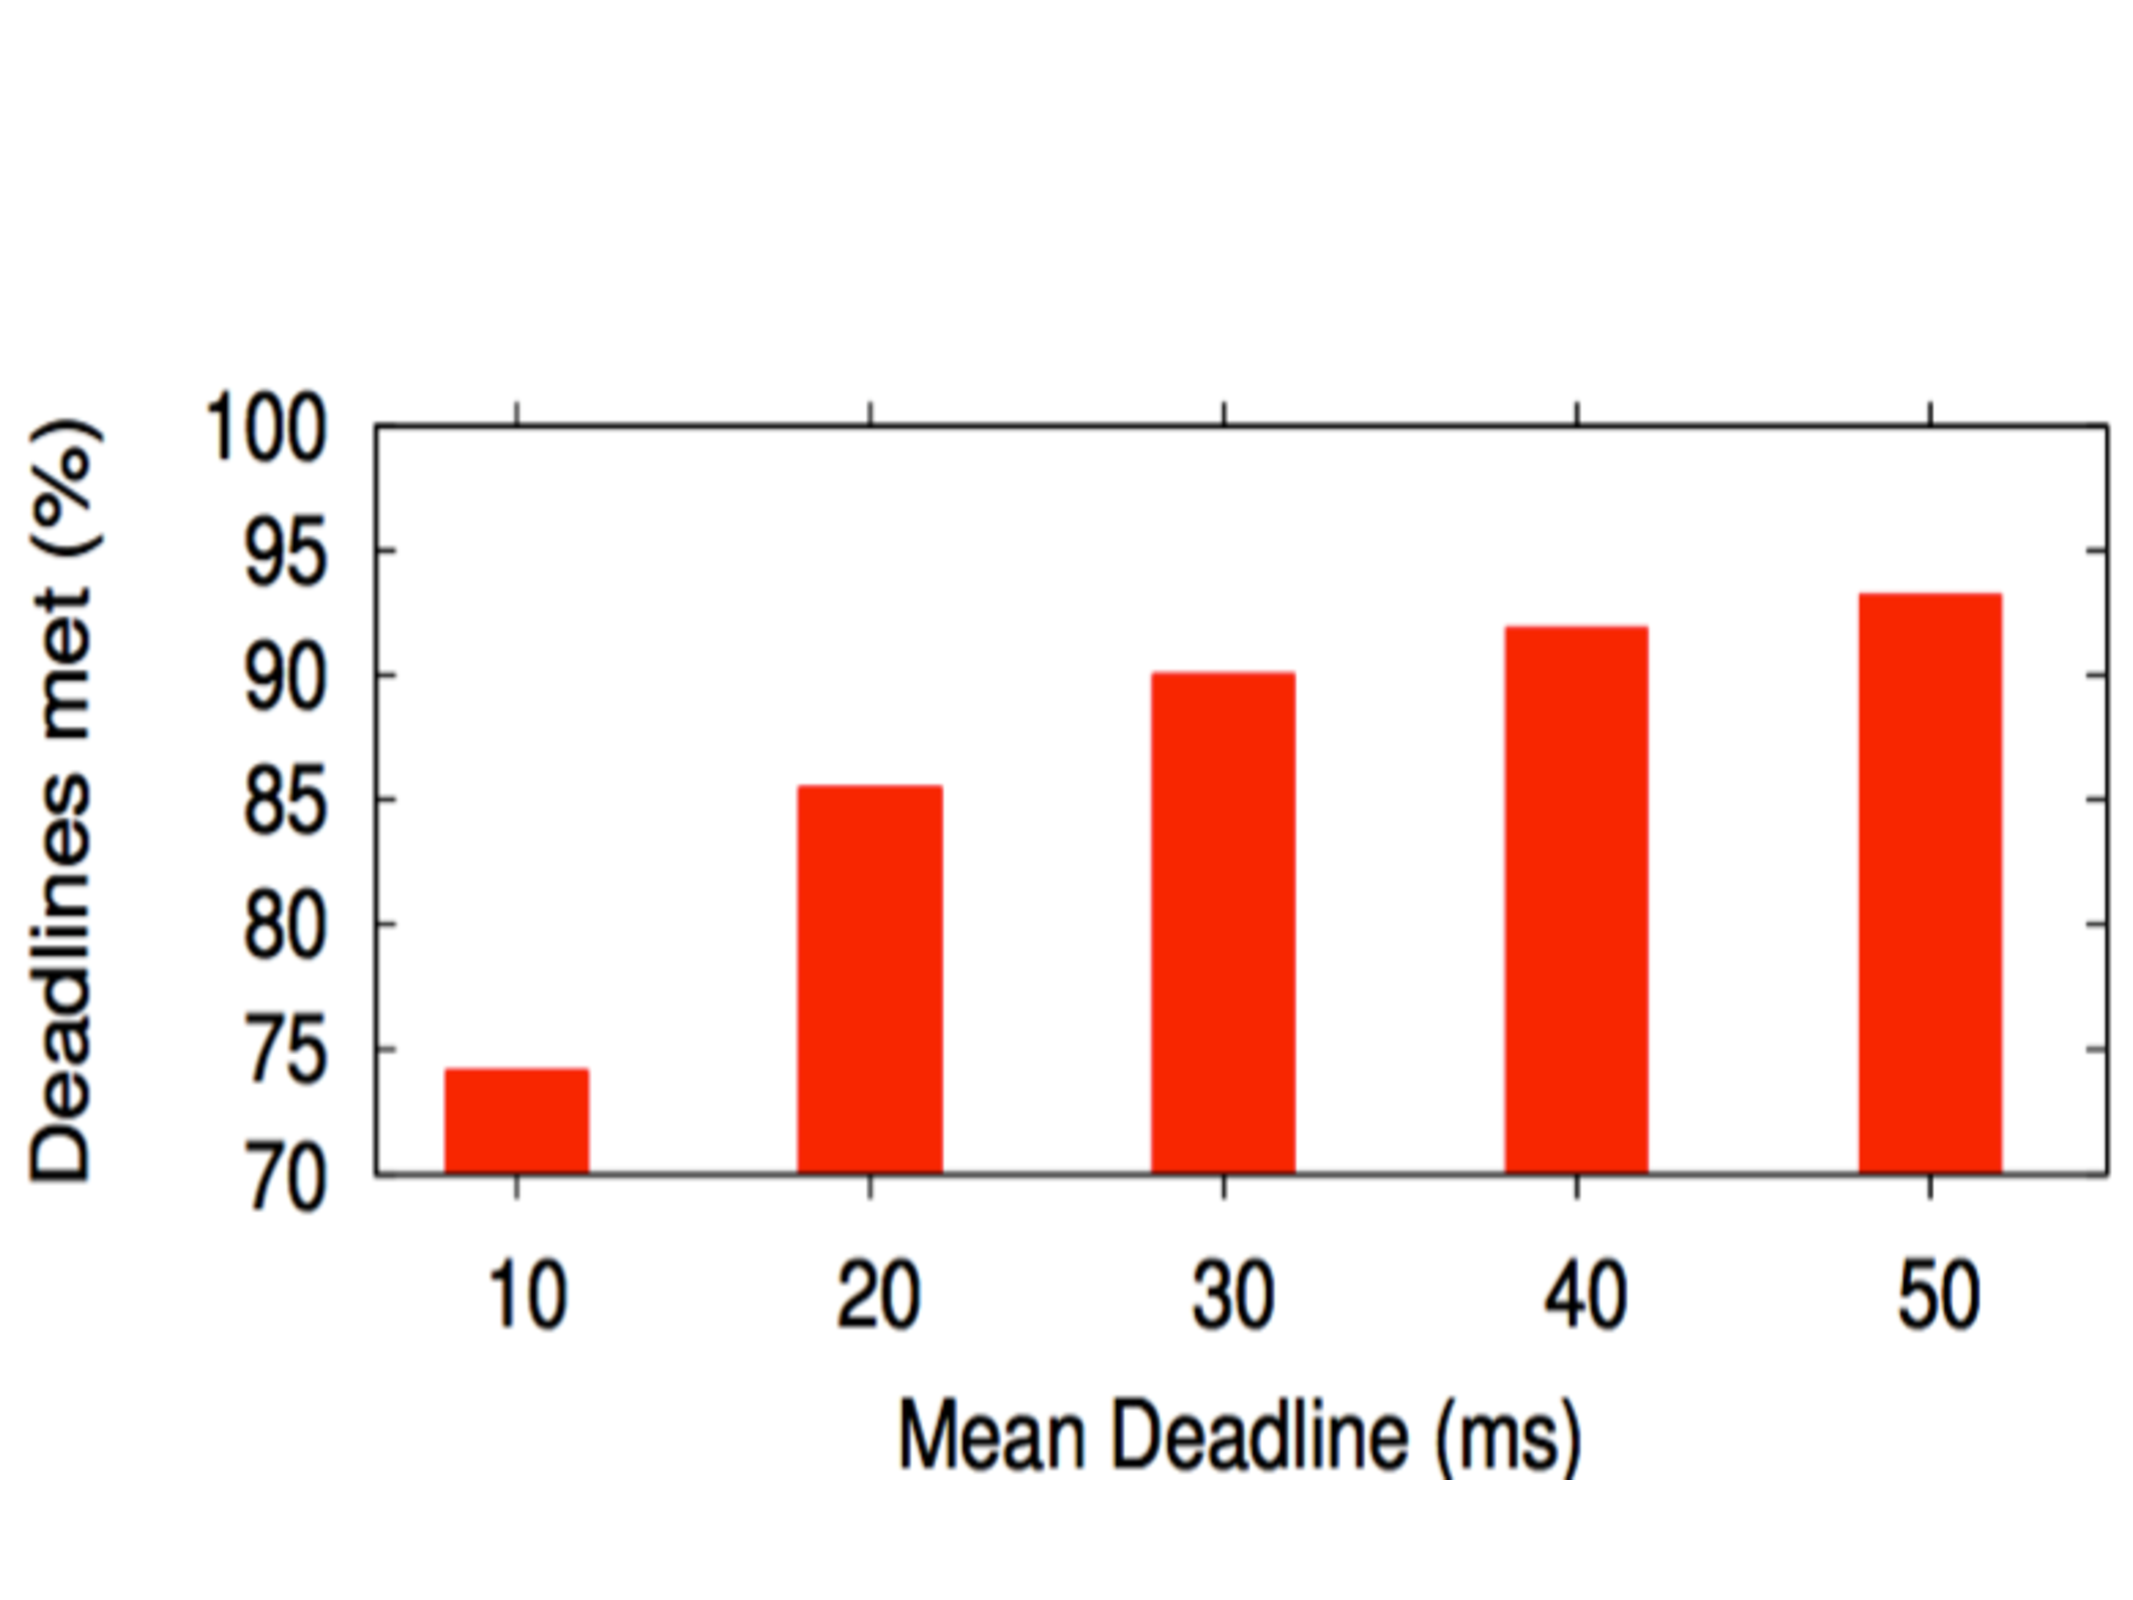
\includegraphics [width=0.9\columnwidth] {figures/others/deadline-picture.pdf}
\caption{partition-aggregate 模型}
\label{relatedwork-deadline-fig}
\end{center}
\end{figure}

因此,诸如Partition-Aggregate这类模型的SLA (Service Level Agreement)
要求worker等节点的询问和应答传输在截止期限(deadline)之前完成。
任何没有在截止期限之前完成的数据流都被认定错失期限。
错失期限的数据流越多,会有越多的上层计算节点获得不完整的结果,进而影响服务的质量。
此外,在实际中不同的应用的数据流有不同的截止期限,甚至,同一个应用的不同阶段的传输的期限也不相同。
在实际中,数据中心的流包括时间敏感的短消息(50KB到1MB),用于更新节点状态和传输时间长的背景流量(5KB到50MB)等。
这些数据流在节点之间传递,不同业务的数据流具有不同的期限,有的甚至没有期限。
图\ref{relatedwork-deadline-fig}显示的流传输期限分布情形,从中发现,超过$90\%$的数据流的期限在50ms以内。
事实上,数据中心很多在线服务都需要性能保障\cite{Decandia2007Dynamo,Renesse2002Scalable}。
用户的请求,需要满足延迟的需求。
当请求到达时间节点时,
无论计算结果如何,节点都需要把结果反馈给用户,
如果错过了截止期限,应用的性能难以得到保障。



\subsection{TCP传输存在的问题}
TCP是一种面向连接的、可靠的、基于字节流的传输层通信协议。
尽管TCP在Internet中被广泛应用,然而数据中心应用常常需要数据中心网络提供低延迟高带宽。
因为数据中心网络资源有限,因此直接在数据中心使用TCP协议,会存在以下问题。

\subsubsection{Incast问题}
如果很多数据流在短时间内收敛在交换机的同一接口上,数据包可能会耗尽交换机的缓冲区,导致数据包丢失,导致Incast问题\cite{Vasudevan2009Safe}。
发生Incast常常是因为应用采取分区-聚合通信模式,因为在分区-聚合通信模式中,
工作节点常常在较短时间间隔内会发送反馈给上层节点,导致上层节点交换机缓冲区溢出。

迄今为止的实验发现,Incast经常会发生在实际生产环境中,Incast会影响用户体验,从而影响企业的效益。
这是因为,Incast会导致交换机缓冲区过大,从而请求的数据流错过期限。
如果使用TCP协议,则解决Incast问题的方法主要有:
(1)为每个请求增加随机抖动时间。
使用增加抖动时间的方法,可以避免Incast问题,
但是,给每条流增加随机的抖动,会使一些短流增加额外的延迟,从而使数据流错过期限;
(2)把数据流拆分成短流来适应交换机的缓冲区。
使用拆分数据流的方法,会从语意上破坏应用的完整性。
如果某条短流丢弃数据包,会使的整条长流传输不完整,从而破坏应用的性能,进而影响用户的体验。

\subsubsection{交换机缓冲区队列过长}

大多数数据中心的交换机是共享内存,
交换机的所有端口共享交换机存储。
到达交换机接口的数据包被存储到所有接口共享的高速存储器中。
共享池中的内存由内存管理单元动态分配给数据包。
内存管理单元尝试为每个接口分配尽可能多的内存,
如果一个数据包必须排队等待出端口,
但接口已经达到了最大内存分配或者共享池本身已经耗尽,那么数据包就会被丢弃。
构建大型多端口存储器非常昂贵,
所以大多数便宜的交换机都是缓存都很小。

当前计算机网络判断拥塞的方法主要有三种:基于丢包的拥塞控制方法,基于RTT的拥塞控制方法,基于交换机队列长度的拥塞控制方法。
TCP使用基于丢包的拥塞控制方法,当网络中出现拥塞时,交换机的缓冲区会溢出,此时数据包会被丢弃。
当发送端发现有丢包产生时,拥塞窗口会减半,从而减小发送端速率。
如果不发生丢包,TCP的滑动窗口会一直增大,直到占满端口缓冲区。
因此使用TCP协议,会使的交换机缓冲区溢出并且交换机的队列过长,排队延迟高。
数据中心的传输延迟往往$<1ms$,而排队延迟大约$\sim 10ms$\cite{DCTCP},因此排队延迟是数据中心主要延迟。
使用TCP会使排队延迟高,造成用户体验差,进而影响应用性能和收益。
因此在数据中心中,减小队列 长度是减小延迟的有效方法。

\subsubsection{公平分配带来的问题}

\begin{figure}[b]
\begin{center}
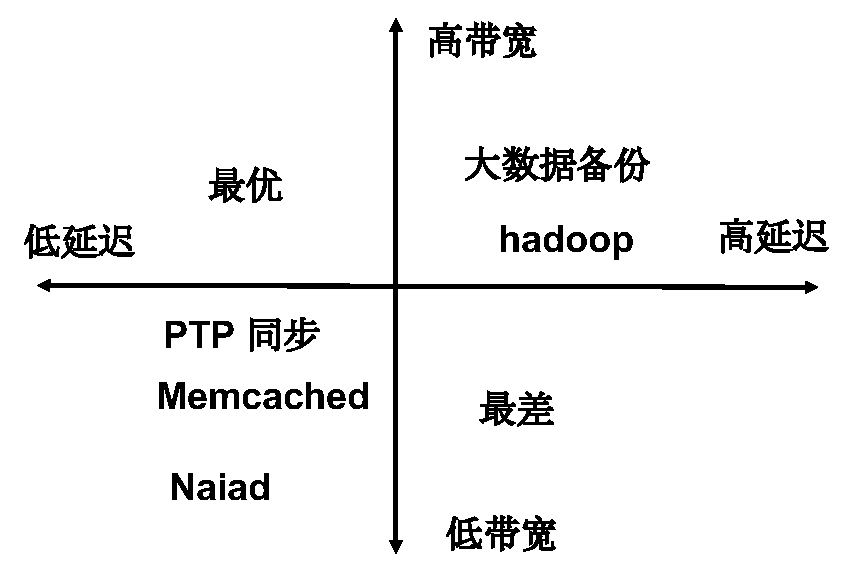
\includegraphics [width=0.9\columnwidth] {figures/others/require.pdf}
\caption{数据中心应用的需求}
\label{relatedwork-require-fig}
\end{center}
\end{figure}


数据中心并存了很多应用,这些应用对带宽和延迟的需求不同,使用TCP策略,带宽服从公平分配的原则。
然而,不同的应用对延迟和带宽需求不同,使用TCP,不能满足所有应用对带宽和延迟的需求。
图\ref{relatedwork-require-fig}显示的是数据中心应用对带宽和延迟的需求,横轴表示的是延迟,纵轴表示的是带宽,
在图\ref{relatedwork-require-fig}坐标系中,从左到右,延迟越来越大,从下到上越来越大。
我们可以看到,对于Hadoop和数据备份,需要高带宽,对延迟需求不大。
对于PTP等应用,对带宽要求不高,但是需要低延迟。
使用TCP协议,对这些应用同等看待,难以满足应用的不同需求,因此,亟需新的方法,考虑应用的不同需求,
智能的分配网络资源,满足应用对网络资源的不同需求。



\section{数据中心网络应用传输方案}
日益使用的数据中心网络尽管有能给应用提供高带宽和低延迟的链路,
 但仍然面临频繁的网络拥塞\cite{Incast08, Incast09}。
传统的TCP协议,难以满足不同的应用对带宽和延迟的需求,针对TCP在数据中心性能不足的问题,业界提出了一系列的方法来弥补。
根据方法优化的粒度,可以分成流级别传输优化方案和任务级别传输优化方案。

\subsection{流级别传输优化方案}
流级别的调度方法,主要侧重提高截止期限前传输完成流的比例,以及优化流的平均完成时间。
从方法上看,流级别的传输优化方法主要可以分成两类,第一种是通过改进传输协议TCP等,调整滑动窗口来调整带宽;
第二种是进行传输调度,采用集中控制的方法,计算流在未来的一个时间段内的传输速率,使的流按照计算出的传输速率进行传输。
本小节,我们从流的传输方法上对流传输进行总结和归类。

\subsubsection{改进TCP的方案} 
在DCN中的许多改进TCP的传输方案中,DCTCP\cite{DCTCP}
提出在交换机的瞬时队列长度超过某个阈值K时,对数据包进行标记,
随后,接收端对被标记的数据包的ACK进行标记,发送端通过统计ACK被标记的比例来计算拥塞程度,
并根据拥塞程度($\alpha$)来调整滑动窗口。
根据拥塞水平$\alpha$,出现拥塞时,滑动窗口变化为w = w$\times$(1 -$\alpha$/ 2)。
通过设置适当的阈值,DCTCP可以使的交换机的队列处于低水平上。
大量的实验表明,DCTCP有效地为短流提供低延迟服务。
然而DCTCP不是根据截止期限进行带宽调整的,
因此对于截止期限敏感的OLDI(Online-Data-Intensive),MapReduce等应用(如网络查询和广告),
DCTCP的调整效果会很差 \cite{D2TCP}。

 D$^2$TCP改进了DCTCP,能更加智能的调整发送端的拥塞窗口。
 它定义了一个期限迫近因子d = T/D,其中T是不采用期限感知的方法,
 传输完成所需要的时间,D是剩余时间。
 出现拥塞时,根据网络拥塞程度$\alpha$和期限迫近因子d的拥塞窗口的调整方法:
$w=w \times (1-\alpha^{d}/2)$。
D$^2$TCP不但具有DCTCP保持排队长度稳定并且队列短的优良特性,
 而且可以使得期限更近的数据流获得更多的带宽。
 D$^2$TCP可以与TCP共存,并且易于在数据中心部署。
 
L$^2$DCT \cite{L2DCT} 尝试减小流完成时间,和D$^2$TCP类似,当出现拥塞时,
L$^2$DCT也使用伽玛校正函数进行滑动窗口调整($cwnd = cwnd*(1-\alpha^{w_c})$)。
L$^2$DCT 近似实现短流优先策略,小的数据流有更高的优先级,因此流平均完成时间变小。
和 D$^2$TCP,DCTCP一样,L$^2$DCT也需要借助网络中ECN的标记。
L$^2$DCT只能够优化流完成时间,而无法优化显式设置期限的数据流。
 
  
TIMELY\cite{mittal2015timely}是基于RTT判断拥塞的协议,
当RTT增大时,TIMELY认为网络中发生了拥塞,发送速率需要降低。
当RTT减小时,TIMELY认为网络拥塞程度轻,可以增大发送速率。
通过RTT进行拥塞判断,TIMELY可以使的交换机队列处于低水平上,从而有效的降低传输延迟。
但是,基于RTT的方法在数据中心存在以下两个问题:首先,数据中心网络中的RTT时间太短,无法准确测量;
而使用RDMA这些新型技术的成本太高。
此外,它不能和基于丢包的策略共存,
因此在实际当中部署存在难度。

ICTCP\cite{ICTCP}通过分析TCP带宽,RTT,和TCP接收窗口(receive window)的关系,
动态的调整TCP接收端的接收窗口(receive window)大小,从而把网络中出现Incast的影响尽量降低。
但是,数据中心RTT的波动大,难以进行测量;
其次,ICTCP侧重于优化网络中的Incast问题,
无法对背景流进行传输优化。

\subsubsection{流调度方案}
 
D$^{3}$ \cite{D3}在集中控制器上计算交换机上所需的带宽,
并把计算的带宽反馈给交换机,使交换机按照计算出的速率发送。
虽然D$^{3}$是第一个已知的基于截止期限进行带宽调整的传输协议,
但是其对数据流优先级调度采用贪心和先到先得的策略,
因此在某些情况下,期限远的数据流会比期限近的数据流优先调度 \cite{D3}。
另一方面,D$^{3}$ 需要修改交换机硬件,因此在实际中部署难度大。

PDQ \cite{PDQ}在端上使用抢占式流量调度来分配带宽。
与D$^{3}$不同,PDQ以分布式方式工作,
其抢占式调度可以处理D$^{3}$无法处理的场景。
PDQ可以使用不同的调度策略,如最早截止期限(Earliest Deadline First,简称EDF)或最短作业优先(Shortest Job First,简称SJF)。
然而,SJF是单一链路上的流平均完成时间最小化的最佳解决方案。
对于复杂链路来说,它并不是最优的。
PDQ使用流平均完成时间被用作评估指标,
PDQ还要求修改交换机的硬件,不能与传统的TCP共存。
 
 PIAS\cite{bai2015information}借助于交换机当中存在的队列, 
 实现了 MLFQ(Multiple Level Feedback Queue )机制。
 在这种机制中,流的优先级开始最高,随着数据发送,
 流的优先级开始降低,PIAS近似实现了短流优先的策略,
 从而间接的优化了流平均完成时间。
 然而PIAS只是优化流平均完成时间,并没有考虑网络拥塞情形,
 当网络拥塞时,并不能满足紧急应用的数据流对带宽的需求。
 
 
QJUMP\cite{grosvenor2015queues}给每个应用分配一个优先级,
对高优先级的应用在发送端进行限速,而一旦数据包进入网络中,
高优先级的数据包可以排在交换机的前列,低优先级的数据包排在交换机队列的后面。
从而实现了高优先级的数据包有较低的延迟,而低优先级的数据包,有更高的网络带宽。
QJUMP在高带宽和低延迟找到了一个平衡,
但是,在实际应用中,应该合理的给应用分配优先级,
如果优先级分配不合理,会导致应用性能降低。
 
 
在FastPass \cite{perry2015fastpass}中,发送端何时发送数据包,
以及发送数据包的路径由中央处理器的计算结果决定。
FastPass借助数据包发送时间算法和数据包发送路径算法来决定数据数据包发送时间和发送路径。
通过这两个算法,FastPass能够在不改变硬件的前提下,
使交换机队列浅,从而降低排队延迟。
FastPass可以有效的降低网络中交换机队列长度,
但是FastPass是集中式控制的方法,集中式控制的方法在数据中心中会增加传输延迟。
此外,如果控制器发生故障,会导致系统崩溃。

pFabric \cite{pFabric}根据流剩余数据量大小进行调度,
pFabric \cite{pFabric}提出的分布式算法近似于最短作业优先(Shortest Job First,简称SJF)策略,
并且被证明在优化流平均完成时间问题上是近似最优策略。
与PDQ相比,pFabric将流量调度与速率控制分离开来,实现起来更加简单,并且可以与类似TCP的方案共存。
pFabric需要单独的交换机,这导致pFabric在网络中难以部署。
 
 
DeTail\cite{DeTail},侧重于跨层技术,
包括流的优先级调度和高效的负载平衡策略,
以减少长流的完成时间的。
尽管能有效的减少网络传输延迟,但是DeTail需要使用新的网络协议,
因此在实际难以大规模使用。


Karuna \cite{chen2016scheduling} 是调度混合流(有期限的流和没有期限的流混合)场景下的解决方案。
Karuna主张,对于有期限的流,要在截止期限之前完成,对于没有截止期限的流,平均流完成时间影响最小。
Karuna \cite{chen2016scheduling} 可以减少流失时间的流量百分比,并减少流的平均完成时间。 
Karuna必须在交换和终端节点上进行改变。
这使得Karuna在实践中部署难度很大。

PASE\cite{PASE}声明的协议(DCTCP,PDQ,pFabric等)不是竞争关系,它们是互补的。
PASE不改变网络中的器件,在减少流完成时间方面性能要比pFabric复杂。
 
\subsection{任务级别传输优化方案}
流级别的传输优化方案,能够优化单条流的完成时间,
或者尽量保证流在截止期限之前完成。
但是,单纯的流级别传输并不能满足应用的需求。
比如web 搜索(分区-聚合模型),数据备份,MapReduce,
分布式存储等应用是包含很多并行的数据流。
对多阶段的应用,只有当上一阶段传输完毕后,下一阶段才能开始传输,
因此,为了应用能够取得更好的性能,需要从流传输任务的级别进行优化。

Orchestra\cite{Chowdhury2011Managing}发现任务传输时间占据了任务总处理时间的33$\%$\cite{Chowdhury2011Managing}。
因此,Orchestra首先提出调度应该侧重优化任务阶段整体传输,而不只是优化某条数据流。
Orchestra使用一个全局的控制器来对所有传输信息进行同步,这个全局控制器存储了所有源和目的节点信息。
对于广播的传输网络传输结构,Orchestra采用Cornet协议,更加合理的利用网络拓扑进行传输优化。
对于shuffle的传输,Orchestra采用权重shuffle调度进行带宽分配。
Orchestra从总体上优化了任务传输,尤其对广播和MapReduce的shuffle阶段性能提升显著。

Barrat\cite{dogar2014decentralized}提出在调度应用的数据传输时,
应该在任务的级别进行,而不是在流级别进行。
Barrat对任务的调度整体采用FIFO模式,对于数据量大的任务,
随着传输进行,降低任务优先级,从而保证大任务不会阻塞链路,影响小任务的传输。
Barrat是一个分布式的任务级别调度系统,
通过对任务的整体调度,Barrat能够有效的减小任务平均完成时间,同时减少任务最长的传输延迟,
进而提升应用的传输性能。


Varys\cite{chowdhury2014efficient}提出对于存在数据并行的应用,
应该以coflow\cite{chowdhury2012coflow}为调度单元,而仅仅在流级别进行优化是不够的。
Varys提出对应用的优化的目标是最小化平均流组(coflow)完成时间。
为了达到这个目标,Varys采用集中式调度策略,首先计算流组的优先级,然后计算每条数据流的带宽。
对于流组优先级,Varys采用最小瓶颈优先(Smallest-Effective-Bottleneck-First,简称SEBF)启发式算法来决定。
最小瓶颈优先策略策略是把一个流组(coflow)中传输最慢的流的完成时间当做流组的预估完成时间,
然后根据预估传输时间进行排序,使得预估完成时间小的流组获得高优先级。
对于数据流的带宽的控制,使用最小带宽期望(Minimum-Allocation-for-Desired-Duration,简称MADD)算法。
使用集中控制的方法,借助以上两个策略,Varys优化了平均流组完成时间(Coflow Completion Time,简称CCT),从而提高了应用的性能。

Varys需要预先得知很多流组(coflow)的信息,
事实上,在数据中心中,很多应用的流组(coflow)中流的大小信息是很难预先得知的,尤其在hadoop多阶段计算中,
中间shuffle会传输大量数据,数据流的大小很难被预先得知。
基于此,Aalo\cite{chowdhury2015efficient}提出,在调度coflow时,应假设预先不知流组(coflow)中流的大小进行调度。
Aalo实现了最短流组优先策略 ,
根据已经发送数据量的大小,把流组(coflow) 分配到不同的优先级队列中。
相同的优先级队列中的流组(coflow)采取FIFO调度机制。
Aalo近似实现最短流组(coflow)优先的策略,整体上调度了流组(coflow),从而优化了流组(coflow)的传输效率。

事实上,无论Aalo还是Varys,都需要提前分别出应用的流组(coflow),这需要对应用进行改动。
而修正比如Hadoop和Spark等应用的API需要考虑兼容性和进行Java-byte级别的改动,这导致修改的复杂度较高。
CODA\cite{zhang2016coda}首先尝试不改变应用,来自动的区分和调度应用流组(coflow)。
同时使用late binding等措施来尽量减少流组(coflow)区分的错误等。
通过对应用的流组(coflow)进行有效的区分和带宽的调度,
CODA从整体上对coflow实现了调度,从而,有效的降低了应用流组(coflow)的传输时间,优化了应用传输延迟。


和Varys,以及Aalo等相同,D-CAS\cite{luo2016towards}将数据网络假设成非阻塞交换机,
认为传输冲突只发生在交换机的入端口以及出端口,中间路径并没有拥塞发生。
D-CAS提出coflow最小化平均传输完成时间调度问题和开放商店中任务平均工作完成时间问题的优化等价。
为了优化coflow传输延迟,D-CAS改进了开放商店中的任务平均完成时间的2-近似算法\cite{roemer2006note},
并将2-近似调度算法引入到流组(coflow)的调度中,然后改进2-近似调度策略,从而得到流组(coflow)的在线调度算法。
D-CAS采用分布式的方法实现,可以有效的减小流组(coflow)的传输时间。



RAPIER\cite{zhao2015rapier}打破了数据中心非阻塞体系结构,
认为在传输中,拥塞随时发生,不只发生在第一跳和最后一跳。
传输时不应只考虑调度问题,为每条数据流分配合理的路径是很重要的问题。
基于此,RAPIER把流组(coflow)的路径选择和流组(coflow)的调度放在一起考虑,
通过求解非整数优化问题,把每条数据流发送速率的大小和发送路径都计算出来。
RAPIER可以减少平均CCT在50$\%$以上,并且易于在真实环境中部署。
和Varys相同,RAPIER需要预先得知coflow中每条数据流大小等信息。


Task-aware TCP\cite{liu2017task}认为传统的TCP-based方法只考虑了单一流的情形,
而没有考虑流之间的关系,这会影响流之间的传输,导致传输效率低。
Task-aware TCP主张,在一个task中,速率过快的数据流应该把带宽让给速率慢的数据流。
Task-aware TCP\cite{liu2017task}改进了DCTCP方法,借助于ECN标记,区分出传输过快和传输过慢的数据流,
把传输过快的数据流带宽给传输过慢的数据流一些,
从而使的任务的平均传输时间减少,进而优化了任务的传输延迟。




Qiu在\cite{qiu2015minimizing}从理论角度考虑有权重的流组(coflow)的调度,
假设已经知道coflow到达时间,每条流的信息进行调度。
Qiu同时强调调度流组(coflow)时,应该也同时考虑权重,而不应该把所有流组(coflow)同等看待。
使用近似算法,Qiu提出的策略,可以达到$\frac{67}{3}$的近似比。
使用随机性策略,算法的近似度可以达到$9+16\frac{\sqrt{2}}{3}$。
Qiu在\cite{qiu2015minimizing}通过求解方程组对流组(coflow)进行调度求解,此方法有较高的复杂度,
在实际中难以部署。


\subsection{数据中心传输方案存在的问题}
相比于传统的TCP,当前数据中心传输方案能够有效的提高数据中心传输效率,
提高应用对网络等资源的使用情况,
然而,尽管数据中心网络技术在不断发展,
但是,随着应用业务的不断发展,数据中心网络始终难以满足应用的各种需求,
因此,需要更加合理的网络资源调度来满足应用对网络资源的需求。
当前数据中心网络依然存在以下的问题:

\textbf{(1)未考虑网络拥塞程度和应用传输期限关系}

D$^3$首先提出,在进行传输时,
应该给数据流分配足够多带宽,让数据流满足期限。
D$^3$改动交换机,并在交换机上计算出数据流传输满足期限的最小带宽,
从而数据流能够获得足够多的带宽,从而在期限之前完成。
D$^2$TCP根据网络的拥塞情形和数据流期限调整数发送窗口,
通过拥塞窗口间接的影响数据流传输的带宽,进而实现不同需求的数据流达到各自传输的目的。
这两种方法都同时考虑了数据流传输的期限和网络拥塞状况。
然而,无论哪种方法,都没有考虑网络拥塞程度,期限的二维关系。
事实上,尽管D$^2$TCP考虑了数据流的传输应该同时考虑网络期限,
但是当网络拥塞程度严重时,D$^2$TCP不再是基于期限调整的拥塞控制策略。
因此,如何合理的根据网络拥塞情形,期限调整数据流传输是亟需解决的问题。


\textbf{(2)无法同时满足延迟敏感流和带宽敏感流的需求}

数据中心中同时存在对延迟敏感的短流和对带宽敏感的背景流。
当前的数据中心的传输方案,无论是D$^2$TCP,
D$^3$还是L$^2$DCT都是解决单一数据流的需求,
即或者满足延迟敏感流的需求,或者满足带宽敏感流的需求,
比如D$^2$TCP,D$^3$侧重优化有显式期限的流,
L$^2$DCT优化的是流平均完成时间,
并不能同时满足这两种数据流的需求。

\textbf{(3)任务级别调度只考虑网络拥塞并没有考虑任务的重要性}

尽管Varys,Aalo等策略在调度数据中心资源时,
是在任务级别进行的,
但是这些策略只是考虑网络的拥塞状况,
目标是优化应用的传输完成时间。
然而,应用有不同的语意,只考虑应用的传输是不够的,应该同时兼顾应用的重要性。
比如,进行计算的hadoop和视频传输业务共享数据中心资源,
进行计算的hadoop的业务的优先级比进行视频传输业务的优先级高,
使用传统的传输策略,会认为这两个应用数据流的优先级相同,
这样常会导致进行计算的Hadoop业务的数据流得到的带宽不足,
造成Hadoop的完成时间过长,从而影响应用的整体性能并且造成网络资源利用率偏低。

基于以上的几个问题,本文从流级别和任务级别对传输策略进行优化和改进,
使的流的带宽能够根据网络拥塞和流的期限进行动态调整,
同时对混合场景下的流传输进行优化,
使有期限的数据流和对带宽敏感的数据流都能满足需求。
最后从任务级别对传输进行了优化。

\section{本章小结}
本章中,我们综述了数据中心应用传输方案的相关工作。
我们从常见应用的通信模型和数据流量等方面对数据中心传输进行了概述。
然后,我们总结了流级别和任务级别的数据中心传输方案进行。
最后,我们总结了数据中心传输方案存在的问题。














